\chapter{Detectors Test, Alignment and Calibration.} \label{analysis}
\commento{
\begin{outline}[enumerate]
\1 development of the analysis program.
\1 testing the analysis program with montecarlo data.
\1 Test of the detectors in the Lab.
\1 Beam line description.
\1 Data Analysis
	\2 thresholds scan
	\2 Rates on $Pb^{208}$.
	\2 Beam related asymmetry correction.
	\2 $C^{12}$ Asymmetry.
\end{outline}}

\paragraph{}
In this chapter we discuss the electronic test that have been carried out in the laboratory, and the calibrations that need to be done
in order to calculate, from the raw data, the final data ready for the analysis.
The test in the lab consist in checking that the photo-multipliers are working and that the electronics that take care of acquiring the data do not have any errors.
For the calibrations, since several beam parameters are needed for the analysis, it's important to obtain the correct scaling factor to convert the Raw Data collected by the \textit{VFC}s to data with the right physical units. The important quantities are the $X,Y$ impact point coordinates of the beam,the energy $E$, the beam current $I$ and the scattering angles $\theta_{x}$ and $\theta_{y}$.

\section{Data Tree Implementation}

Referring to the next picture, we now discuss briefly the structure of the data that is implemented in the analysis program, this is important to clarify how data analysis will be developed:

\begin{figure}[hbtp]
\centering
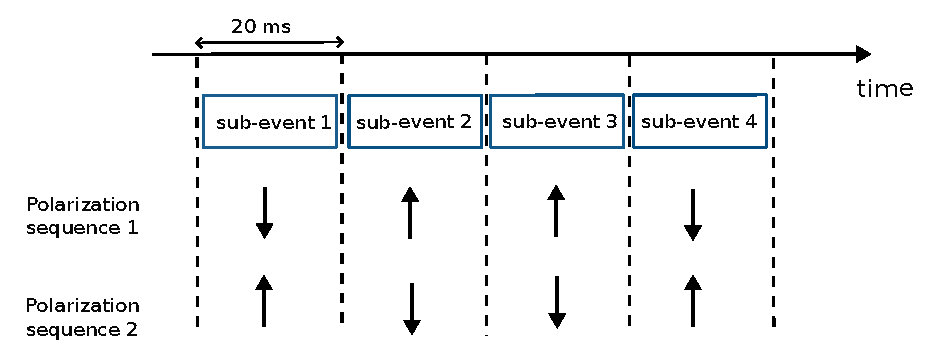
\includegraphics[width = 0.75\textwidth]{ExperimentalSetup/EventStructure.pdf}
\caption{}
\end{figure}

The base class that is implemented in the analysis program is the \textit{Event} class. As we mention above in \ref{FirstDescription}, we do not intend to keep track of the single scattered electron, instead we analyze time series of $\SI{80}{\milli \second}$, in which we simply count all the electrons detected in this time interval. The work-flow of the analysis program is load the binary file collected during the beam time, parsing  one event at a time and processing the raw-data from the beam monitors and the detectors. During the execution of the program data files in \textit{.txt} are generated and filled with the processed data ready. The output data-file can be analyzed with any software package, such as root or python, to get the value of the asymmetry $A_{n}$. 
The picture shows that every event is divided into $4$ sub-events. For each different sub-event a precise state of the polarization is defined, 
$+1$ for $S = \uparrow$ and $-1$ for $S = \downarrow$. Every sub-event is $\SI{20}{\milli \second}$ long; during this time interval master-board receives all the data coming from the monitors and the detectors and sent them to the data-acquisition program (DAQ) that produces the binary-files, which are the input of the main analy\begin{figure}[hbtp]

\centering
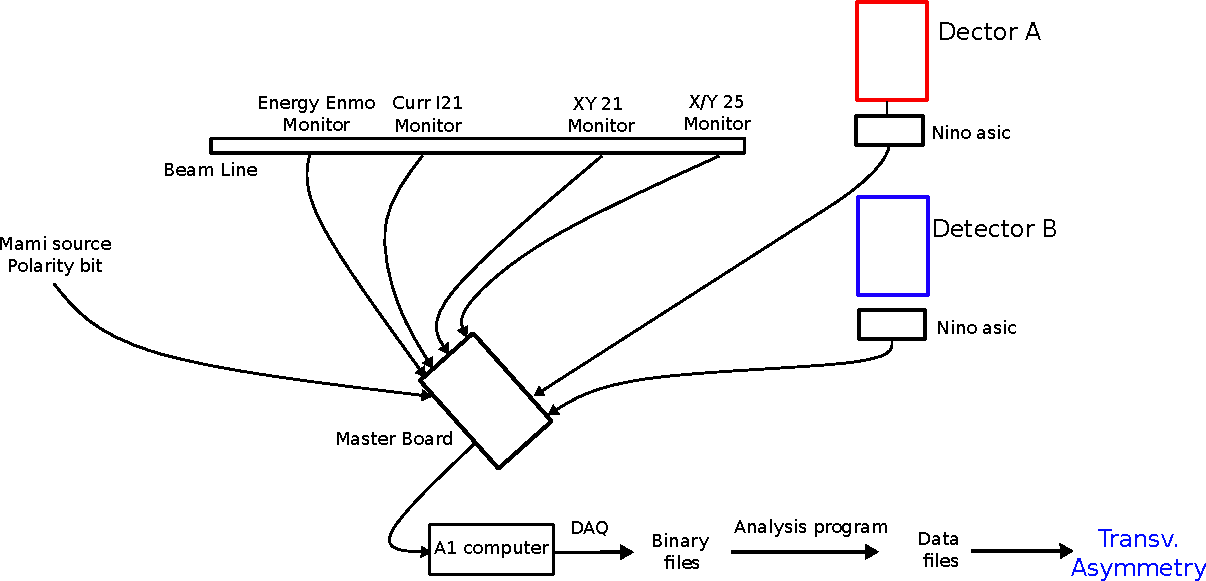
\includegraphics[width = 0.75\textwidth]{Analysis/Electronic_scheme.pdf}
\caption{Scheme of the data flow.}
\end{figure}
sis program.

 It is important to note that for each sub-event, a single measurement is acquired from the beam monitors, which is intended as a time average of the various signals on the 20 milliseconds of sub-event duration. The sampling rate is then equal to $\SI{50}{\hertz}$.

This structure of the data is quite specific for particle physics experiment. The main reason for this setup is connected with the need to avoid as much as possible that the variations of intensity, position and energy of the beams induce an effect that add to $A_{n}$. Considering only small time series, it is assumed that the beam is quite stable, in order to reduce undesired effects.
Nevertheless, the contribution of these effects, which are indicated for brevity as false asymmetries, is considered in the final model.
Several values are saved with the number of scattered electrons, for each event. Here we will present briefly all the various quantities that are saved, and the general structure of the data tree:

\begin{figure}[hbtp]
\centering
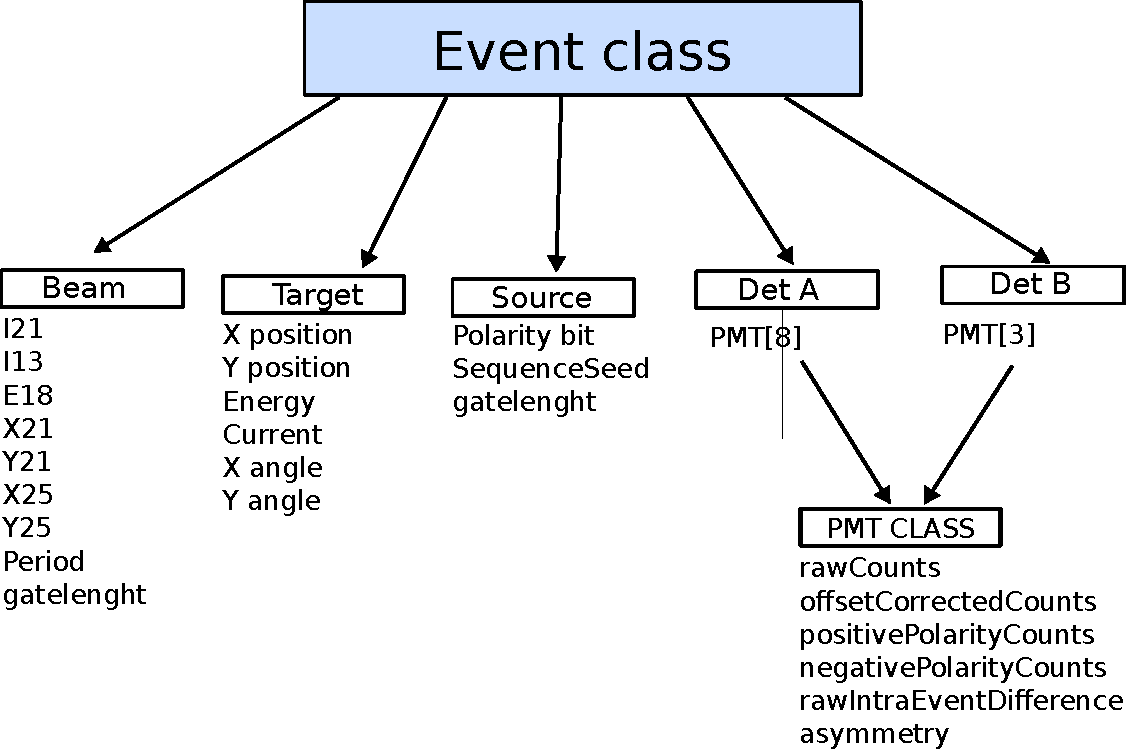
\includegraphics[width = 0.8\textwidth]{Analysis/EventClass.pdf}
\caption{Scheme of the Event class, the structure of the data treen is shown here in a simplified version, for the complete reference see appendix.}
\end{figure}

\section{Nino Board}
In this section we explain briefly simple test that we performed to control that the two detectors are working properly.Before going into detail it is important to describe again the operation of the NINO board, which interfaces directly with detectors.
The Nino board, which digitizes the signal from the PMTS, has two parameters which can be used to select the internal threshold of the discriminator, to cut out the low amplitude signals, that are indicated as threshold and attenuation. The threshold and attenuation values can be adjusted changing the settings of the DAQ program.
For our purpose, we fix the threshold values equal to $600$ for all the detectors. We remind the reader that the values should be in the range ($0,4000$). 
It is desirable to work with the "physical" values, i.e switch from these arbitrary units to the correct value in $\SI{}{\milli \volt}$. The relation between attenuation and threshold it is not linear, the reason is that the NINO board is designed in such a way that collects the input charge coming from the signal. In principle it is even not possible to define a unique value for the threshold in $\SI{}{\milli \volt}$, because signals that produce the same charge can have shape and amplitude different from each other. In simple word, from the definition of the current:

\begin{align}
Q = I \, \cdot \, time
\end{align}

Signal with a large time width and a small amplitude can generate the same accumulation of charge respect to narrow signal with high voltage amplitude. Despite this, some data have been acquired by the A1 collaboration, with which it's possible to define a raw conversion function from attenuation units to threshold. The basic idea is to fix th time-length and the shape of signal and vary the amplitude, then we can observe the minimum value of attenuation for which the NINO board collects the input signal. We are aware that for electrons that hit the detectors, the shape of the signal cold different, and are not fixed, however this procedure let us to have at least a first rough estimate of the threshold value.

\begin{figure}[hbtp]
\centering
\subfloat[][\emph{Threshold dependence against attenuation} \label{fig:ThrvsAtt}]{
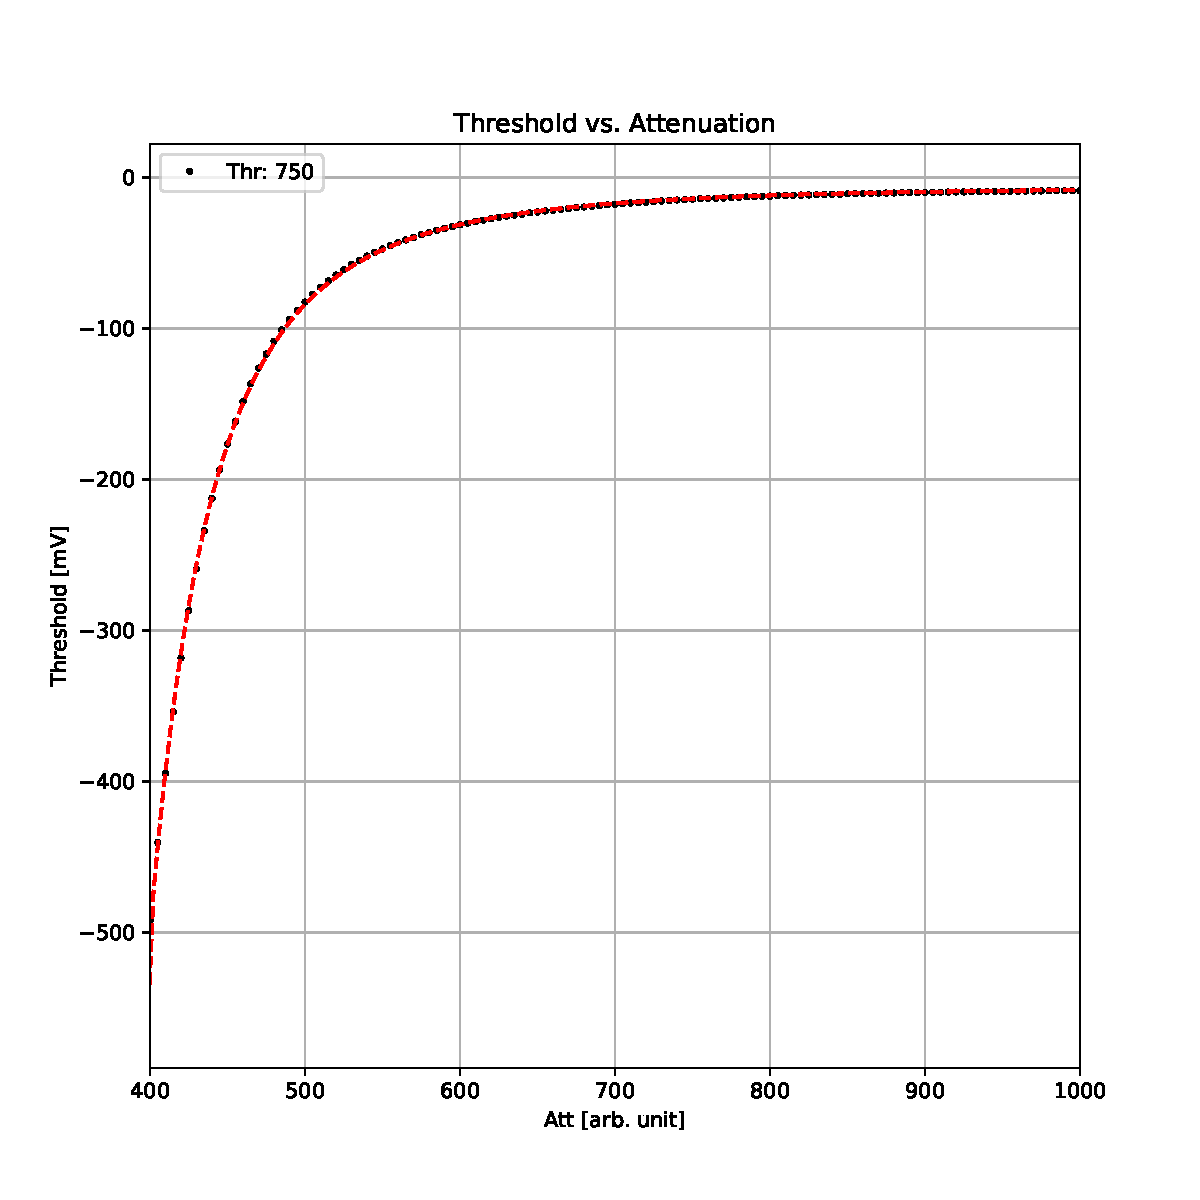
\includegraphics[scale=0.4]{Analysis/Calibrations/ThrvsAtt.pdf}}
\end{figure}

The data show represent the values of the amplitude of the input signals (in $\SI{}{\milli \volt}$) versus attenuation, the function used for the conversion is obtained from the fit of the data, the function used is the following: 

\begin{equation}
Threshold = \dfrac{a}{(att - b)^{3}} + c
\end{equation}

The values obtained from the fit are:

\begin{itemize}
\item $a = - 802111053 \, \frac{\SI{}{\milli \volt}}{[arb.unit]}$
\item $b = 382 \, [arb. unit]$
\item $c =  \SI{-6.1}{\milli \volt}$
\end{itemize}

\section{Detector Test}

Before the Beam time, some test with the two detectors were performed, to check that the pmts were still working after some years of inactivity, and that the new electronic was able to count properly the pulses and store the data. For this studies, we didn't have a radioactive sources to employ, so we moved the two detectors in the workshop of the accelerator, and we use the cosmic rays rate as a probe. 

Knowing that the expected number of event for cosmic rays is about $1 \frac{event}{\SI{}{\centi \meter\squared} \SI{}{\second}}$ we can compute the expected values for the number of events. We decided to take 1 minute long acquisition for both the two detectors, this leads to $70$ expected events for detector B  and  $100$ events for detector A.  \smallskip

The first step is to select a good point of work for the threshold. So, fixing the value of the threshold parameter for the NINO board, we took several acquisitions, each of them one minute long, increasing each time the attenuation. We powered the pmts with a negative voltage around $ \SI{-1000}{\volt}$, as suggested in the data-sheets, and covered the cherenkov detector with a shielding blanket, to avoid ambient light simulating a signal.

\begin{figure}[hbtp]
\centering
\subfloat[][\emph{Attenuation scan for Detector B}]{
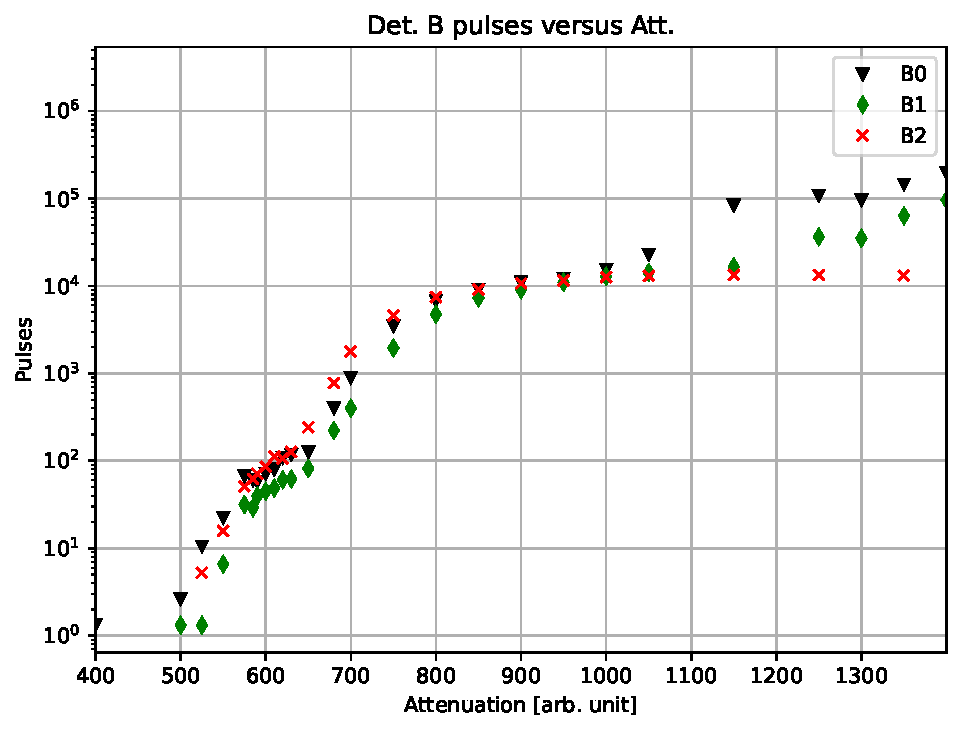
\includegraphics[width = 0.45\textwidth]{Analysis/AttenuationB.pdf}}
\end{figure}

We observed a small knee in the plot, around the zone of 580 − 600 of attenuation, where the number of counts was almost constant, roughly equal to the number of expected events from muons hitting the detector. Then we observe a big edge for attenuation = 1000. Looking at the plot \ref{fig:ThrvsAtt}, we assume that the attenuation values are so high that electronic noise is no longer rejected, in fact the counts grow enormously. The attenuation was set at 600.

The next step was to study the statistical fluctuation of the counts, so we collected 10 acquisitions, each of them 1 min long. The measured values are reported in the table below:

\begin{center}
\begin{tabular}{|c|c|c|c|}
\hline 
Pmt: & 1 & 2 & 3 \\ 
1 & 58 & 60 & 62 \\ 
\hline 
2 & 62 & 55 & 59 \\ 
\hline 
3 & 61 & 59 & 70 \\ 
\hline 
4 & 73 & 66 & 70 \\ 
\hline 
5 & 68 & 66 & 56 \\ 
\hline 
6 & 59 & 52 & 64 \\ 
\hline 
7 & 69 & 74 & 77 \\ 
\hline 
8 & 48 & 49 & 57  \\ 
\hline 
9 & 70 & 54 & 58 \\ 
\hline 
10 & 60 & 61 & 66\\
\hline
\end{tabular} 
\end{center}

This data are interesting to check if the counts are following the theoretical distribution of the events expected for cosmic rays at sea level. If the pmt are working in a good mode, we know that the number of counts should be Poisson-distributed:

\begin{equation}
Pdf(\mu,k) =  \frac{\mu^{k}}{k!} e^{-\mu}
\end{equation}

The variance of the Poisson distribution is equal to the mean of the counts, and we expect the same behaviour also for the sample mean and the sample variance:

\begin{align*}
\begin{split}
\mu_{1} = 62.8	\qquad \sigma^{2}_{1} = 54.40 \qquad r_{12} = 0.66\\
\mu_{2} = 59.6	\qquad \sigma^{2}_{2} = 57.15 \qquad r_{23} = 0.65\\
\mu_{3} = 63.9	\qquad \sigma^{2}_{3} = 46.98 \qquad r_{13} = 0.35 \\
\end{split}
\end{align*}

We report also the correlation $r_{xy}$ between the pmt. The result are fine: we are able to see a positive correlation between adjacent pmt, and as expected the correlation is lower in the case of the more distant. This is explained by the lower probability that the photons of Cherenkov radiation light up at the same time pmts that are far away from each other.
We can test that the data follow a Poisson distribution using the well-known Gosset test, defined as:

\begin{equation}
\chi^{2}_{n-1} = \sum_{i = 1}^{n} \dfrac{(Oss_{i} - Att_{i})}{Att_{i}}
\end{equation}

We report the result obtained with the data for detector B, the test shows that there is good agreement with the hypothesis that the count are Poisson-distributed.

\begingroup
\setlength{\tabcolsep}{8pt} % Default value: 6pt
\renewcommand{\arraystretch}{1.2} % Default value: 1
\begin{center}
\begin{tabular}{|c|c|c|c|}
\hline 
Pmt: & 1 & 2 & 3 \\ 
\hline
$\chi^{2}_{9}$ & 8.52 & 8.45 & 6.37 \\ 
\hline
\end{tabular} 
\end{center}
\endgroup

To convince oneself that the pmt are actually measuring signals given by the passage of cosmic rays, and not only noise, we placed one pmt in coincidence with the others. If we are able to observe positive correlation between the counts, we conclude that the signal comes from the same event.

\begin{center}
\begin{tabular}{|c|c|c|c|c|}
\hline 
pmt & 0 & 1 & 2 & 4 (in coincidence) \\ 
\hline 
1 & 63 & 57 & 72 & 28 \\ 
\hline 
2 & 55 & 51 & 64 & 18 \\ 
\hline 
3 & 62 & 53 & 75 & 27 \\ 
\hline 
4 & 71 & 62 & 75 & 33 \\ 
\hline 
5 & 68 & 59 & 49 & 23 \\ 
\hline 
6 & 57 & 55 & 63 & 18 \\ 
\hline 
7 & 70 & 64 & 64 & 24 \\ 
\hline 
8 & 50 & 69 & 69 & 25 \\ 
\hline 
9 & 65 & 62 & 62 & 19 \\ 
\hline 
10 & 74 & 71 & 77 & 28 \\ 
\hline 
\end{tabular} 
\end{center} 

As above, we report the sample mean, the variance and the correlation between the pmt in coincidence and the detector B:

\begin{equation*}
\begin{split}
\mu_{0} = 63.5 \qquad \sigma^{2} = 58.9 \qquad r_{04} = 0.49 \\
\mu_{1} = 60.3 \qquad \sigma^{2} = 43.3 \qquad r_{14} = 0.38 \\
\mu_{2} = 67.0 \qquad \sigma^{2} = 71.1 \qquad r_{24} = 0.65 \\
\end{split}
\end{equation*}

The pmt number 4, that is the pmt in coincidence with the detector, was placed geometrically over the pmt number 2. 
We observe a positive correlation for the values $r_{04},r_{14},r_{24}$, the correlation is higher for the pmt number 2, and less for 0 and 1, for a geometrical reason. \smallskip

\begingroup
\setlength{\tabcolsep}{8pt} % Default value: 6pt
\renewcommand{\arraystretch}{1.2} % Default value: 1
\begin{center}
\begin{tabular}{|c|c|c|c|c|}
\hline 
Pmt: & 1 & 2 & 3 & pmt in coincidence \\ 
\hline
$\chi^{2}_{9}$ & 8.95 & 6.44 & 10.96 & 9.52\\ 
\hline
\end{tabular} 
\end{center}
\endgroup
\smallskip

\commento{We also check at the oscilloscope if we were able to observe three negative peaks at the same time: 
\begin{figure}
\centering
\includegraphics[width = 0.5\textwidth]{Analysis/IMG_20221027_170925.jpg} 
\caption{Signal shape at the oscilloscope, we observed the coincidence between the three pmts.}
\end{figure}}

The same procedure was followed also for detector A. We analyzed 4 signal at a time, because during these lab test we had only one NINO board, with only 4 channels available.
\begin{figure}[hbtp]
\centering
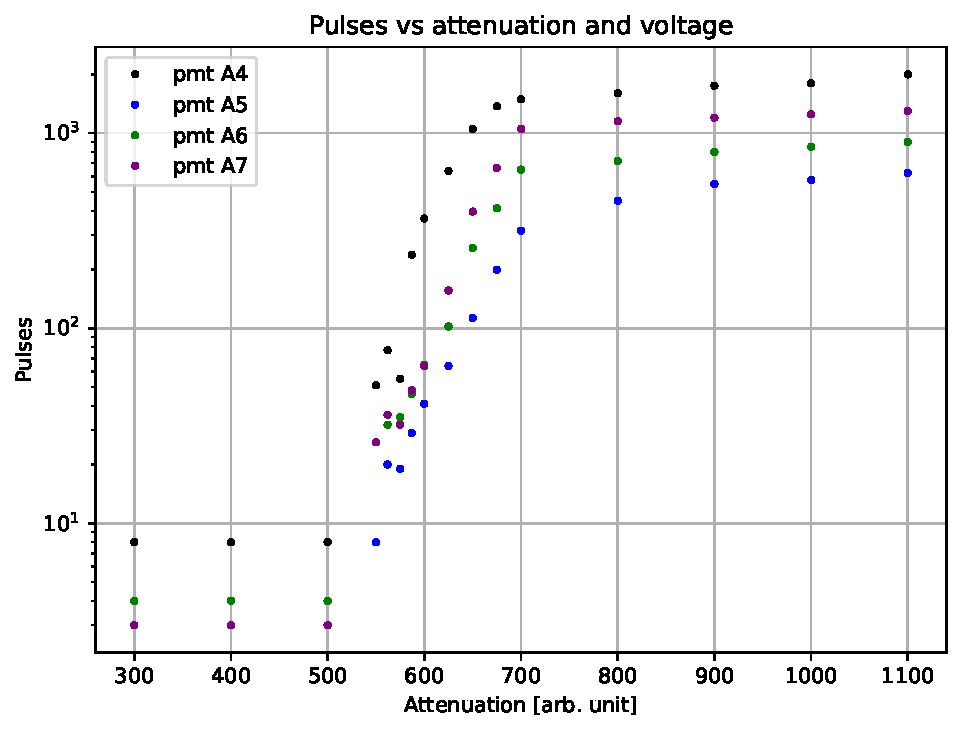
\includegraphics[width = 0.5\textwidth]{Analysis/AttenuationA(4-7).pdf}
\caption{Attenuation scan for Detector A, for the pmt 4-5-6-7}
\end{figure}

We repeat the same test of detector B also for this 4 pmts, without finding any problem or strange behavior. The same procedure was repeated also for the last 3 Pmts of detector A, we took as above 10 acquisitions 1 minute long to study the count distribution, with one pmt in coincidence:

\begin{center}
\begin{tabular}{|c|c|c|c|c|}
\hline 
pmt & 2 & 1 & 0 & (in coincidence) \\ 
\hline 
1 & 91 & 51 & 50 & 27 \\ 
\hline 
2 & 86 & 61 & 50 & 7 \\ 
\hline 
3 & 58 & 48 & 45 & 18 \\ 
\hline 
4 & 95 & 62 & 41 & 29 \\ 
\hline 
5 & 69 & 60 & 50 & 21 \\ 
\hline 
6 & 85 & 57 & 45 & 19 \\ 
\hline 
7 & 66 & 51 & 46 & 28 \\ 
\hline 
8 & 74 & 51 & 48 & 22 \\ 
\hline 
9 & 77 & 43 & 45 & 17 \\ 
\hline 
10 & 62 & 44 & 50 & 29 \\ 
\hline 
\end{tabular} 
\end{center}

\begin{equation*}
\begin{split}
\mu_{2} = 76.3 \qquad \sigma^{2} = 160  \\
\mu_{1} = 52.8 \qquad \sigma^{2} = 47.5 \\
\mu_{0} = 47.0 \qquad \sigma^{2} = 9.6  \\
\mu_{4} = 21.7 \qquad \sigma^{2} = 48.2 \\
\end{split}
\end{equation*}

For these 4 pmts, $\sigma^{2}$ is different from the expected mean, this doesn't agree with the hypothesis that the count are Poisson distributed, we can quantify this with a statistical test: in this table the correlation matrix:

\begingroup
\setlength{\tabcolsep}{8pt} % Default value: 6pt
\renewcommand{\arraystretch}{1.2} % Default value: 1
\begin{center}
\begin{tabular}{|c|c|c|c|c|}
\hline 
Pmt: & 2 & 1 & 0 & pmt in coincidence \\ 
\hline
$\chi^{2}_{9}$ & 19.6 & 8.30 & 1.90 & 39.5\\ 
\hline
\end{tabular} 
\end{center}
\endgroup
\smallskip

The expected error for the result of this test is $\sigma = \sqrt{2*(n-1)} \simeq 4$. In this case we are observing 3 values that are more than  $3 \cdot \sigma$ far from the expected value. If we look at the correlation matrix :

\begin{center}
\begin{tabular}{|c|c|c|c|c|}
\hline 
pmt: & c & 0 & 1 & 2 \\ 
\hline 
c 	 & 1 & -0.18  & -0.21  & -0.06  \\ 
\hline 
0 	 & -0.18  & 1 & -0.10  & -0.22  \\ 
\hline 
1    & -0.21  & -0.10  & 1 & 0.56  \\ 
\hline 
2    & -0.06 & -0.22  & 0.56  & 1 \\ 
\hline 
\end{tabular} 
\end{center}


We observe negative correlation between the pmts, something not expected. After some investigations, we find out that the program which controls the NINO board had a bug: the program partially overwrote some detector B settings for detector A as well. Since detector B has only three pmt's, the problem affected the PMT's with the same numbering as detector A. After fixing this issue we repeated the same test, without finding any problem. 

\section{Calibration}

For the \transv on $^{12}C$ represent an ideal test for the new electronic system. Previous measurements of the $A_{n}$ have been performed at MAMI for carbon target (\cite{}). For this beam-time, the red spectrometer is placed at the angle of $+22.5^{\circ}$, and the blue one at $-22.5^{\circ}$, respect to the longitudinal direction. For these two angle, we have the same kinematics and $Q^{2}$ values of the previous measurement. The exact values are reported here: 

\begin{flushleft}
\begin{align*}
& det. A : \qquad Q^{2} = \SI{0.041337}{\giga \electronvolt \squared} \qquad \textnormal{without Cut} \\
& det. A : \qquad Q^{2} = \SI{0.0394513}{\giga \electronvolt \squared} \qquad \textnormal{with Cut} \\
& det. B : \qquad Q^{2} = \SI{0.0404771}{\giga \electronvolt \squared} \qquad \textnormal{without Cut} \\
& det. B : \qquad Q^{2} = \SI{0.0405843}{\giga \electronvolt \squared} \qquad \textnormal{with Cut} 
\end{align*} 
\end{flushleft}

The $Q^{2}$ values is the same of the last measurement performed at MAMI, and is measured with and without rejecting the inelastic electrons. 

\subsection{Alignment of the Scattering Plane.}

\subsection{Beam Monitor Calibration, XY Monitor}

For the calibration of the X Y monitors, special target are used. In the target frame (\ref{fig:targetFrame}) there are two targets made by three carbon wires that are at a fixed distance each other, horizontally and vertically aligned. The distance between the center of the two external wires is measured, and it is equal to $ d_{horizontal} = \SI{2.38}{\milli \meter}$ for the horizontal wires and $d_{vertical} = \SI{2.33}{\milli \meter}$ for the other one.
The procedure to retrieve the correct scaling factor, to convert from the raw-data in $\SI{}{\volt}$ to $\SI{}{\micro \meter}$, is the following: we ask MAMI operators to slowly change the beam position, in the horizontal and vertical direction for the horizontal and vertical target. The beam position can be changed by varying the Magnetic field produced by the \textit{Wobbler 16} magnets (\ref{fig:BeamLine}). 
During this slow variation, our detectors are measuring the rates of scattered electrons, that increase when the beam hit one of the three wires and and decrease when the beam is centered between two wires. We plot the detector counts versus the $XY$ monitors values, in voltage, and we estimate the position given in voltage of the two external peaks. This values can be used, together with the distance $d_{horizontal};d_{vertical}$ already measured, to compute the scaling factors. This procedure is repeated for $X21/Y21$ and $X25/Y25$ monitors.


\begin{figure}[htb]
%\setlength{\columnsep}{10pt}%
\centering
\includegraphics[width = 0.40\textwidth]{ExperimentalSetup/target.pdf}
\caption{Target frame installed during the experiment, on the top we have the two targets made by three carbon wires that are used to calibrate the positions monitors. Then the carbon target and the two lead targets.}
\label{fig:targetFrame}
\end{figure}

Looking at the PMT counts, we observe that the counts increase to a maximum, that is reached when the beam spot is centered on the carbon wire, and then decrease until the next carbon wire is hit by the beam.\\
We plot the pmt data \textit{versus} the $X25,X21,Y25,Y21$, given in $\SI{}{\volt}$. 
Given that we know the real distance between the two external wires, we can obtain the correct scaling factors to calculate the X and Y position from the voltage values. To identify the three peaks in of the carbon target, we fit the data using a gaussian model (see \ref{fig:HorizontalCalibration}). The mean $\mu$ represents the center of the wire, given in $\SI{}{\volt}$.


\begin{figure}[hbtp]
\centering
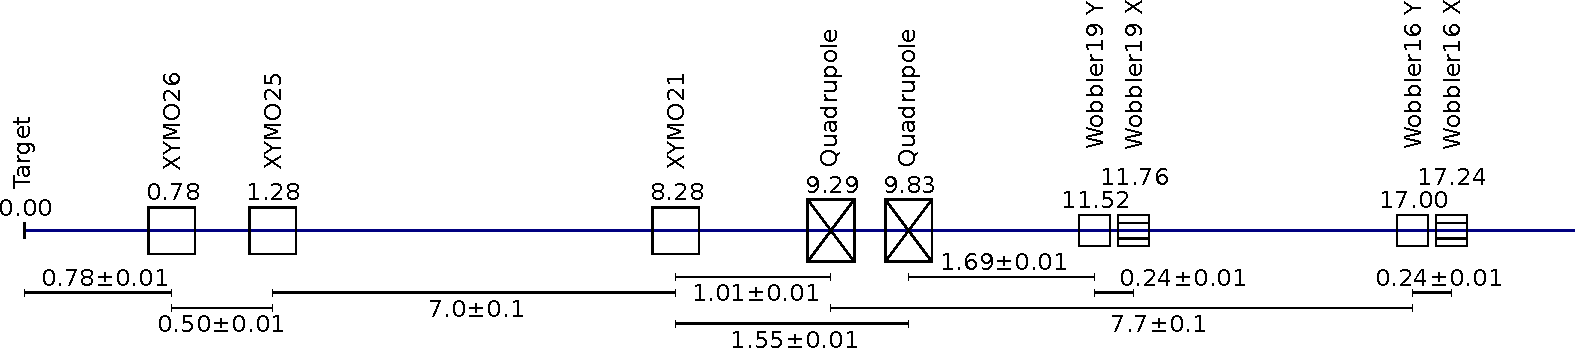
\includegraphics[scale=0.4]{figures/XYMOCalibBeamLine.pdf}
\caption{Beam line scheme.}
\label{fig:BeamLine}
\end{figure}


Looking at the Beam line, we assume that the beam travels in a straight line. Let's consider the \textit{Wobbler 16} magnet the "$0$" of a coordinate system, with the $z$ axis pointing to the target (left direction in the beam scheme). The Beam parameters are measured by the Monitors $X/Y_{21}, X/Y_{25}$, which are located at some distance respect to the target. Suppose we are working only with the $Y_{25}$ monitor (the procedure is the same for the others). The Beam $y$ position is described by:

\begin{align*}
y_{beam} = m \cdot (z - z_{wobbler 16})
\end{align*}

In the scheme \ref{fig:BeamLine} we easily compute the distance between the $Y_{25}$ monitor and the \textit{wobbler 16} magnet, so we have the slope $m$. The Position on the target is given by $Y_{target} = m \cdot Z_{target}$. With these simple equations then:

\begin{equation}
c_{Y25} = \dfrac{d_{vertical} [\SI{}{\milli \meter}]}{ Y_{target}} 
\end{equation}

$c_{Y25}$ indicates the scaling factor of the monitor. With these values the Analysis program compute the correct beam position, and from that the incident angles in the $x,y$ directions, which are needed later for the analysis.

\begin{figure}[hbtp]
\centering
\subfloat[][]{
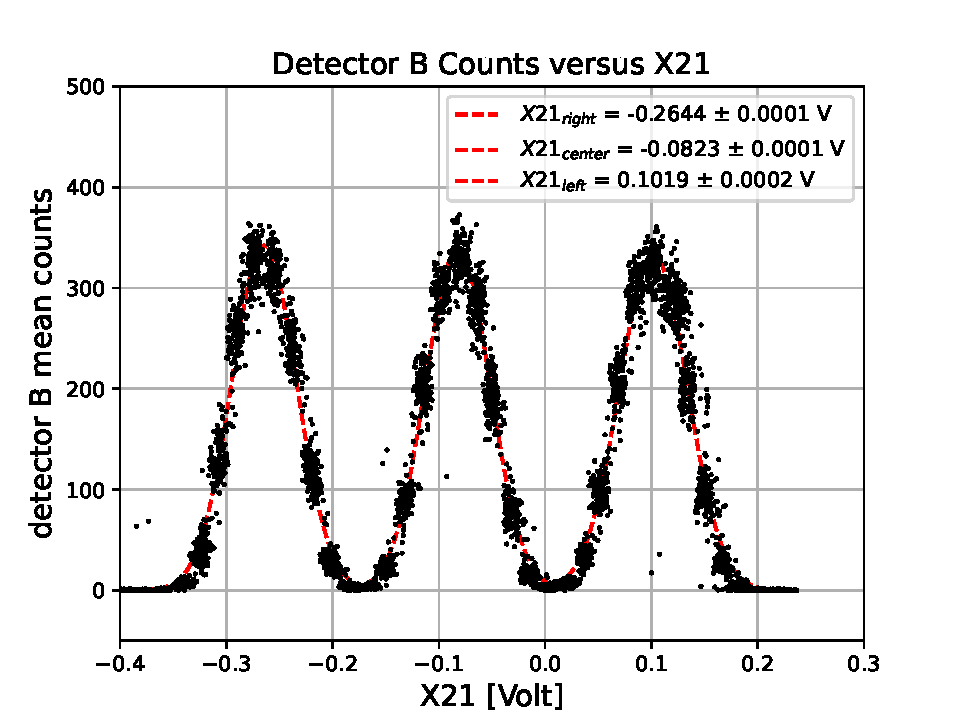
\includegraphics[width=0.4\textwidth]{Analysis/HorizontalCalibration.pdf}}
\subfloat[][]{
\includegraphics[width=0.4\textwidth]{Analysis/HorizontalCalibrationX25.pdf}}
\caption{Plot of the averaged count of detector B, with the slow variations of the beam position in the horizontal direction. The three peaks occur when the beam is aligned with the center of the wire. The values on the X axis are in $\SI{}{\volt}$}
\label{fig:HorizontalCalibration}
\end{figure}

All this procedure can be  checked if we plot now the $X$ and $Y$ position for the same two runs of data acquired with the wires. After placing the scaling factors obtained in the standard configuration file, we run the analysis another time and the physical values were computed \ref{fig:CheckHori}

\begin{figure}[hbtp]
\centering
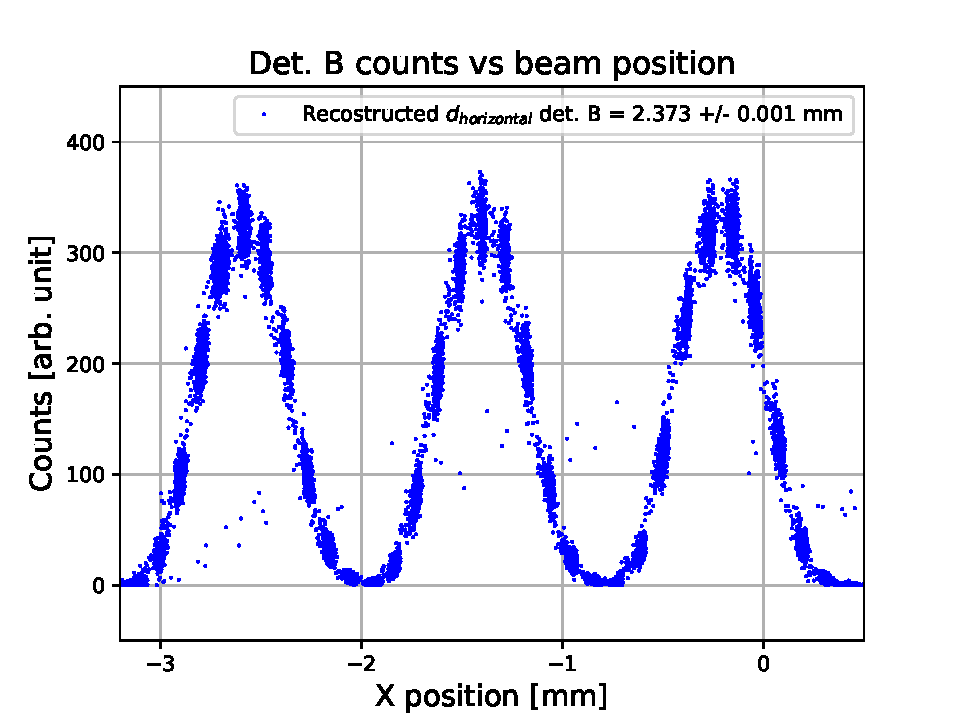
\includegraphics[width=0.45\textwidth]{Analysis/XcheckB.pdf} 
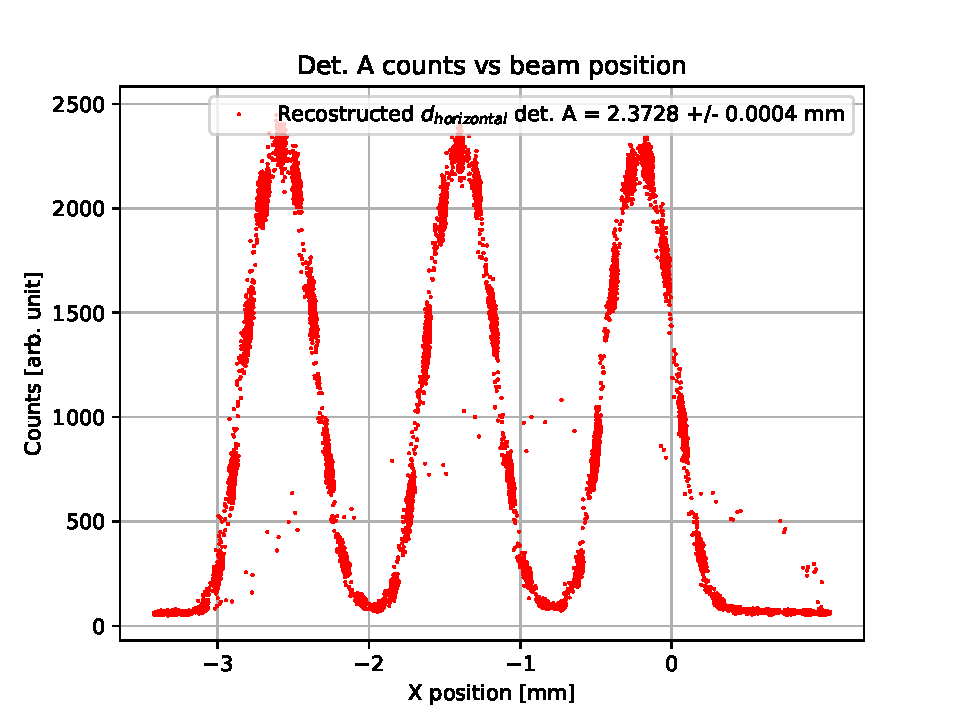
\includegraphics[width=0.45\textwidth]{Analysis/XcheckA.pdf}
\caption{plot of the PMT Count against the physical values computed by the analysis program. Now the position of the three peaks correspond to the expected values measured for the target.}
\label{fig:CheckHori}
\end{figure}
\newpage

\subsection{Current (PIMO) and Energy Monitor (ENMO) calibration.} \label{CurrentCalibration}

The last two calibration needed for the analysis are about the energy and the current intensity of the beam, which are indicated with PIMO (current monitor) and ENMO (energy monitor). 
The values that we measure are given by VFCs counts. We remind the reader how the VFCs monitors operate: the input signal from the beam is transformed in a pulse wave whose frequency is proportional to the input voltage.  The signal is so proportional to various quantities that we want to measure, however we need to determine the correct scaling factor and possible offsets to conver these quantities in physical units ready for the analysis. For this beam time the current is measured in $\SI{}{\micro \ampere}$ and the beam energy is given in $\SI{}{\electronvolt}$.\smallskip

For the current monitors I13 and I21, the raw counts are converted in digitalized voltage values with the formula shown in (\ref{eq:Vfc}). The relation between these values given in $\SI{}{\volt}$ and the real values in $\SI{}{\micro \ampere}$ and $\SI{}{\electronvolt}$ is linear:
\begin{align*}
I(\SI{}{\micro \ampere}) = m I(\SI{}{\volt}) + q
\end{align*}

To determine the two coefficients, the beam current was raised from $\SI{10}{\micro \ampere}$ to $\SI{22}{\micro \ampere}$ in several step. For each step we confront the nominal values of the current with the values in $\SI{}{\volt}$ measured. The following plot show the procedure described:

\begin{figure}[ht]
\centering
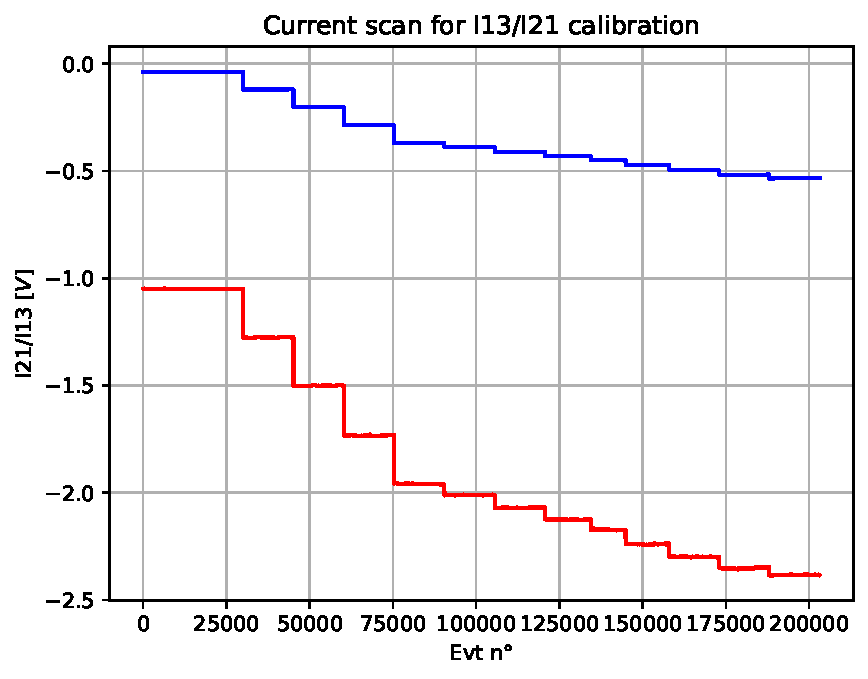
\includegraphics[width = 0.5\textwidth]{Analysis/Calibrations/ScanI21I13.pdf}
\caption{Current scan for the calibration, each step correspond to a run with a different beam current.}
\label{fig:ScanCurrent}
\end{figure}

The calibrations consist in retrieving $m$ and $q$ with a linear fit. Then the parameters are added in the standard configuration file, together with the other calibration parameters, and can be loaded by the analysis program to process the data.  

\begin{figure}[hbtp]
\centering
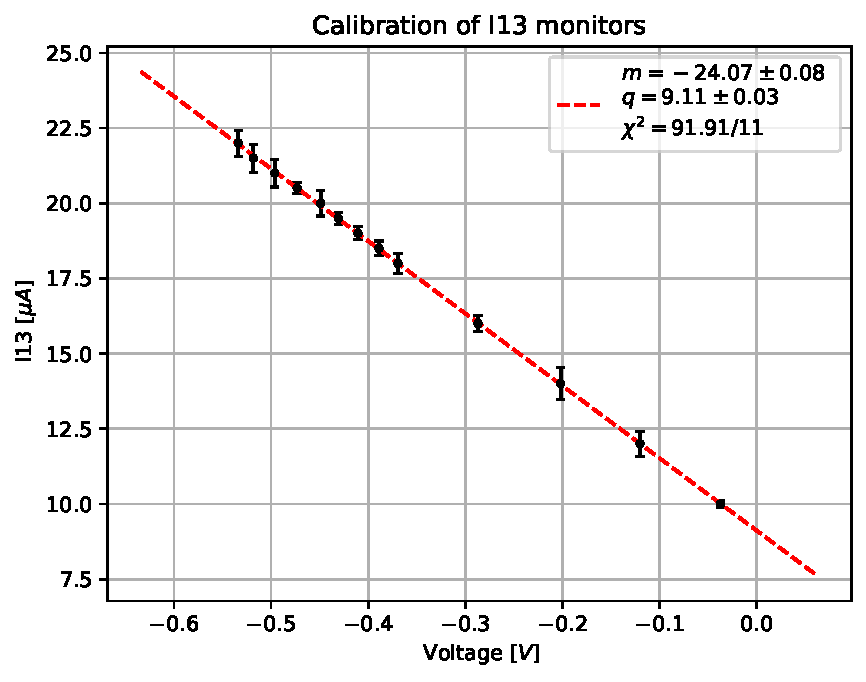
\includegraphics[width = 0.45\textwidth]{Analysis/Calibrations/I13.pdf}
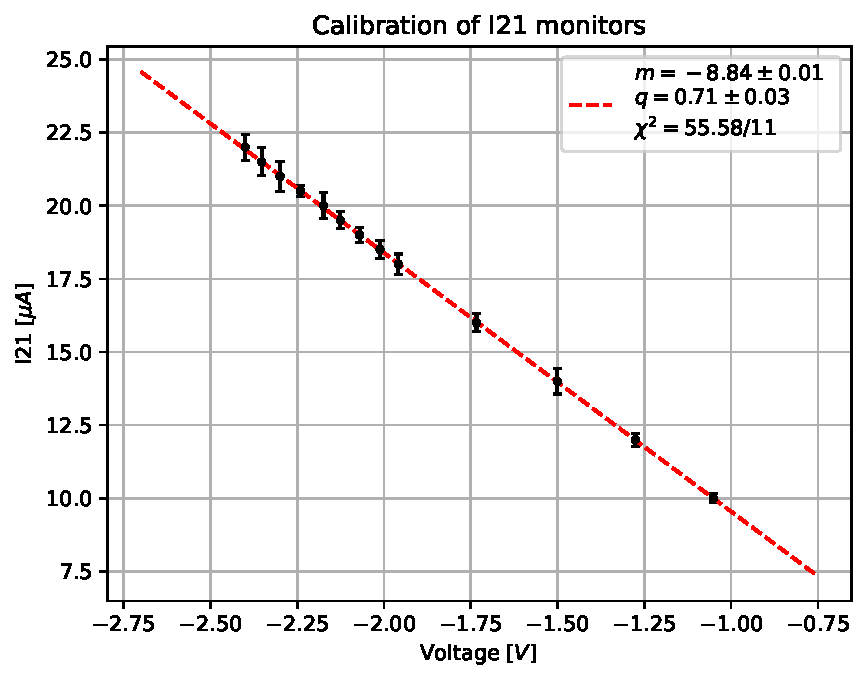
\includegraphics[width = 0.45\textwidth]{Analysis/Calibrations/I21.pdf} 
\caption{Calibrations plots for PIMO I21 and PIMO I13, the errors are multiplied by $25$.}
\label{fig:PimoCalib}
\end{figure}

The values obtained from the fit of nominal beam current vs. voltage values are shown in the figure \ref{fig:PimoCalib}. The $\chi^{2}$ values are higher than the expected. This is not unexpected, the errors in both the plots are computed with the sampling standard deviation formula applied to the sequence of voltage values $I21\/ I13$ ($\sigma_{vfc}$, the standard deviation computed for each step in \ref{fig:ScanCurrent}), and it is related to precision of the analog to digital converter VFCs. The errors are then propagated to the $y$ axis showed in the plot. \smallskip
Yet, we are underestimating the error associated with nominal current $I$, in fact the accuracy associated with the beam current, set by the accelerator operators, was not disclosed, and we suspect that is not negligible compared to $\sigma_{vfc}$. \bigskip  

The ENMO calibration is performed in a different way from the other monitors. The energy calibrations is made with a particular procedure that is automatically made by MAMI operators, and exploit the polarity signal which controls the beam polarization at the source of the acceleration. Mami operators use the signal to create artificially a difference in the beam energy that is correlated to the beam polarity. This difference is equal (nominal) to $\SI{22.6}{\kilo \electronvolt}$, and consist in the last two sub-events with higher energy respect to the first two. Because we know the nominal difference, the calibration consist in computing the correct scaling factor which convert from $\SI{}{\volt}$ to $\SI{}{\kilo \electronvolt}$. The quantity that is relevant for the calibration is $\delta E$ (with $E_{18}$ being the energy monitor):

\begin{equation*}
\delta E = \frac{E_{18}[3] + E_{18}[3]}{2} - \frac{E_{18}[0] + E_{18}[1]}{2} 
\end{equation*}

An histogram of $\delta E$ should show a single peak whose values correspond to $\SI{22.6}{\kilo \electronvolt}$.
For this calibration, we took 3 different acquisition, which differ for the different values of the beam current. We remind that the output voltage signal from the XY monitor is proportional to the current, as mentioned in \ref{eq:SignalToVfc}, so we have that:

\begin{equation}
U[\SI{}{\volt}] = \frac{1}{C_{E18}} \, \cdot  i \cdot E
\end{equation}

So, if we invert the relation we have that:

\begin{equation}
\frac{E}{U} = C_{E18} \, \cdot \frac{1}{i} \qquad  C_{18} = \frac{E}{U} \, \cdot i
\end{equation}  

And we have the scaling factor.

\begin{figure}[hbtp]
\centering
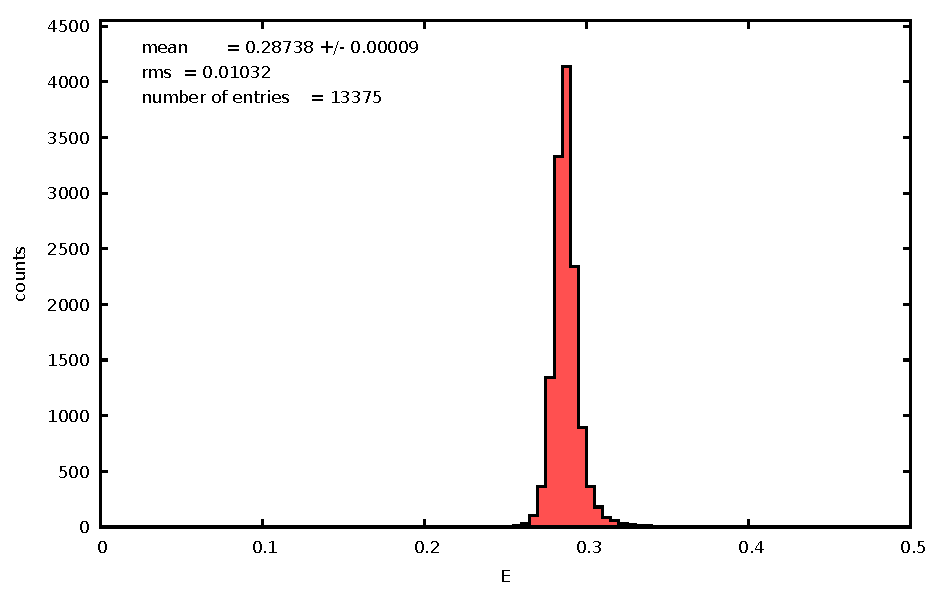
\includegraphics[width = 0.45\textwidth]{Analysis/ENMOvoltage20.pdf}
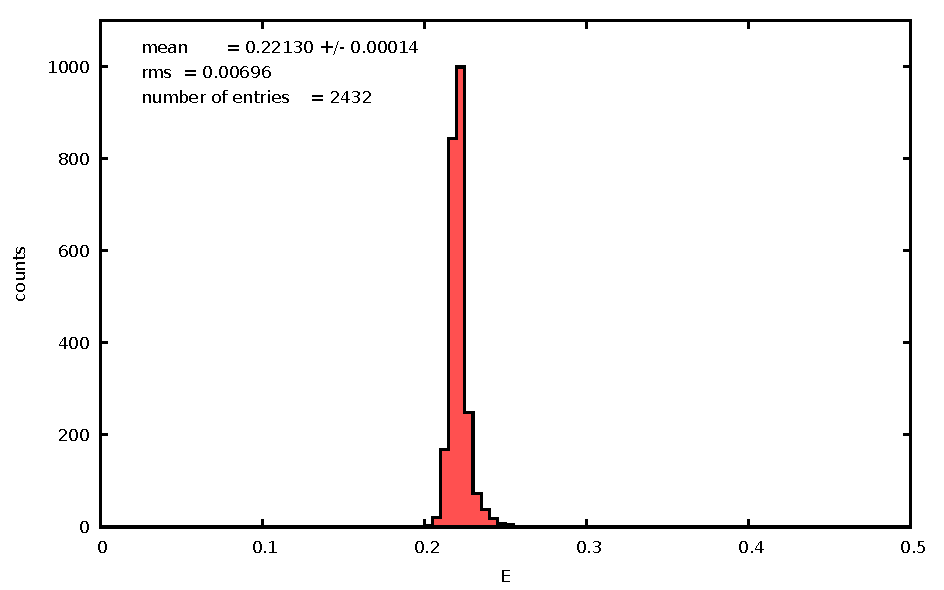
\includegraphics[width = 0.45\textwidth]{Analysis/ENMOvoltage15.pdf} 
\caption{Histograms or $\delta E$ with the beam current $\SI{20}{\micro \ampere}$ on the left and $\SI{15}{\micro \ampere}$ on the right.}
\end{figure}


\begin{figure}[hbtp]
\centering
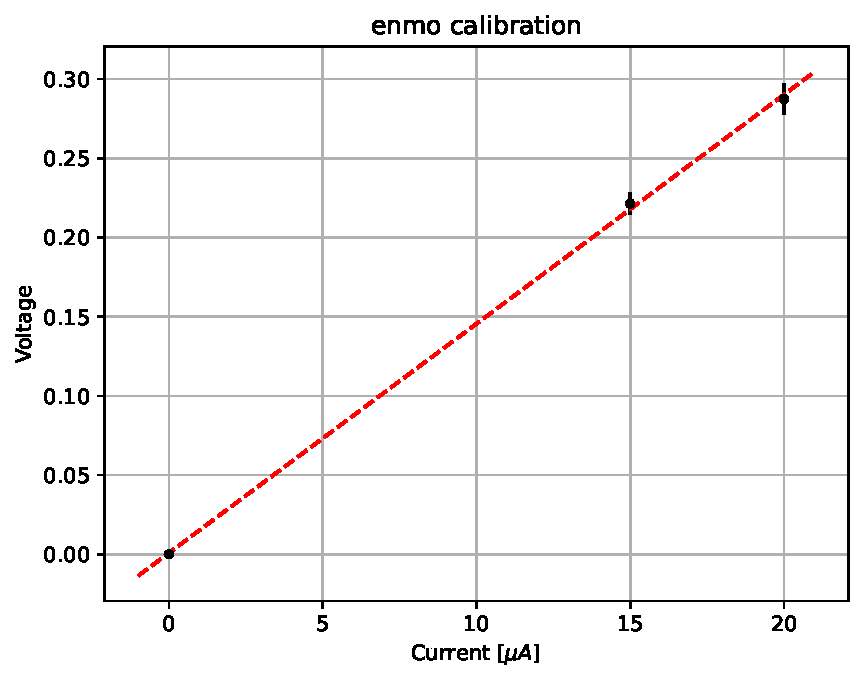
\includegraphics[width = 0.5\textwidth]{Analysis/Calibrations/E18_Calibration.pdf}
\caption{Calibration of ENMO monitor, plot of the ENMO voltage values versus the current.}
\end{figure}


$C_{E18}$ is obtained taking the coefficient parameter $m$ from the fit and substituting in:

\begin{align*}
C_{E18} =  \frac{\SI{22.6}{\kilo \electronvolt}}{m}
\end{align*}

From this we obtain the value $C_{E18} = +1595.2$ necessary to convert from Voltage units to $\SI{}{\kilo \electronvolt}$. Using the value, we can show an histogram of $\delta E$ in physical units, as a check of our procedure:

\begin{figure}[hbtp]
\centering
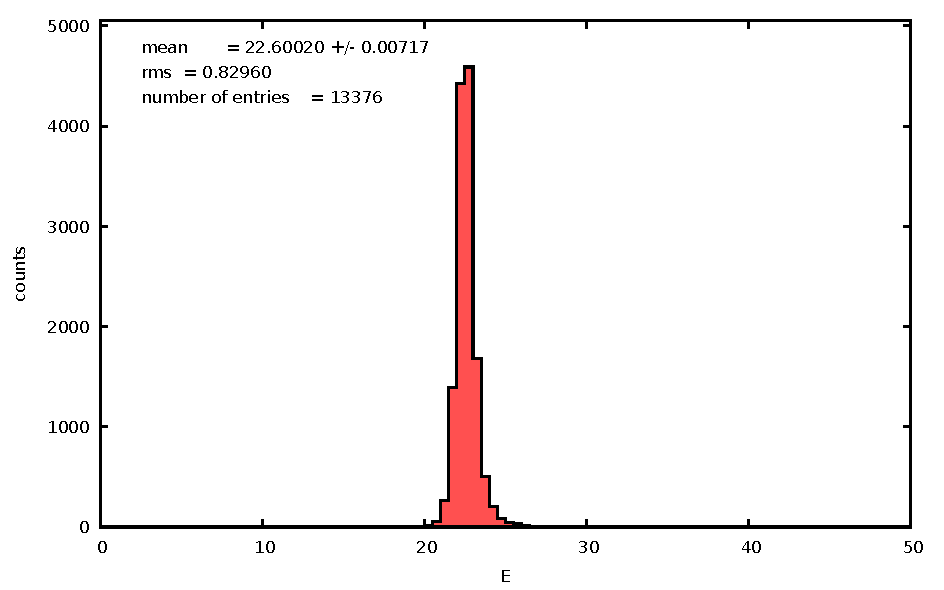
\includegraphics[width = 0.45\textwidth]{Analysis/ENMOCheck20.pdf}
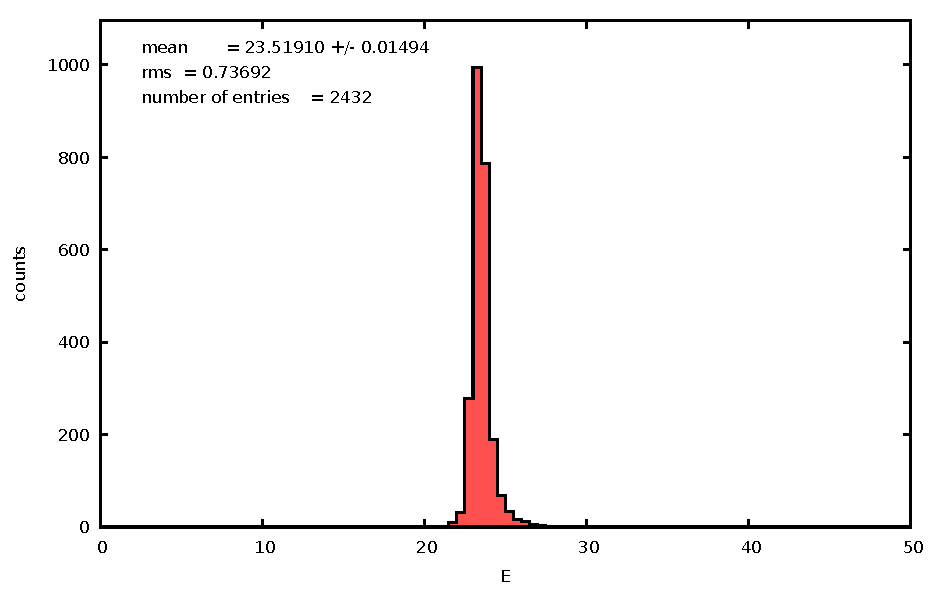
\includegraphics[width = 0.45\textwidth]{Analysis/ENMOCheck15.pdf} 
\caption{Plot for the physical quantities computed in the data tree, for two different current of the beam (on the left $\SI{20}{\micro \ampere}$, $\SI{15}{\micro \ampere}$ on the right)}
\end{figure}
\newpage
\subsection{Calibration of the PMTs}

\commento{Here it's important to show the plots I made during the beam time. I have to mention the Leo tecniques for the correct interpretation of counts vs attenuation.}

During the beam time, several scans in attenuation were performed, before switching MAMI to produce the polarized beam, to choose the best working point for the PMTS of the detectors. The same procedure used in the laboratory was followed, so with a beam intensity of $\SI{10}{\micro \ampere}$ we acquire data run one minute long, increasing each time the attenuation.

\begin{figure}[hbtp]
\centering
\subfloat[][\emph{Attenuation scan for the PMTs of detector B} \label{fig:AttScan}]
{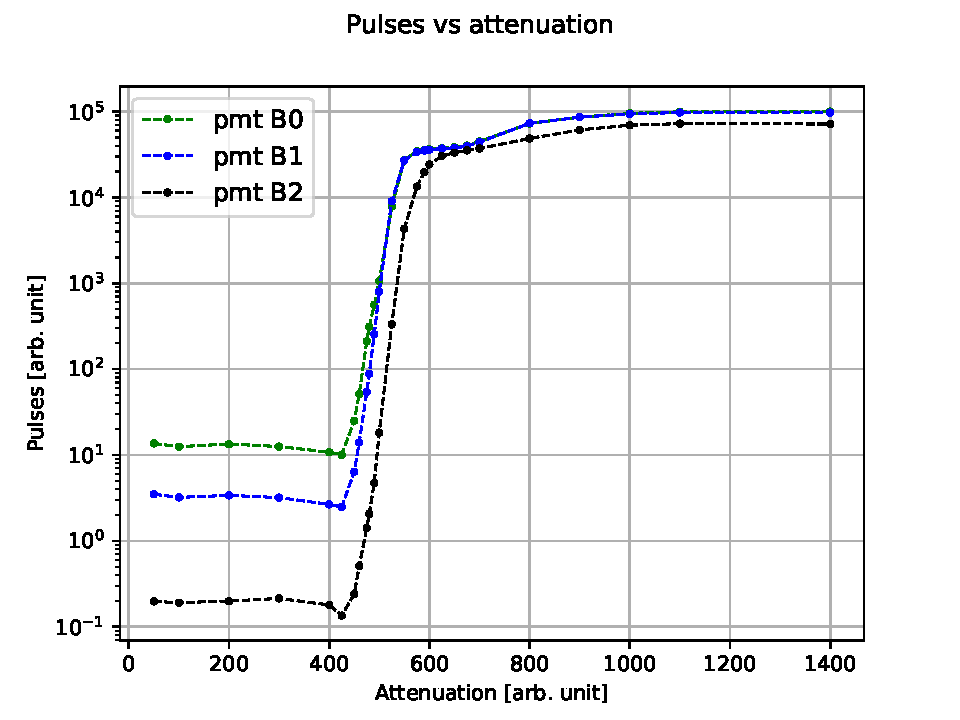
\includegraphics[width = 0.5\textwidth]{Analysis/CalibrationPMT/AttenuationScanB.pdf}}
\subfloat[][\emph{Attenuation scan for the PMTs of detector B}]
{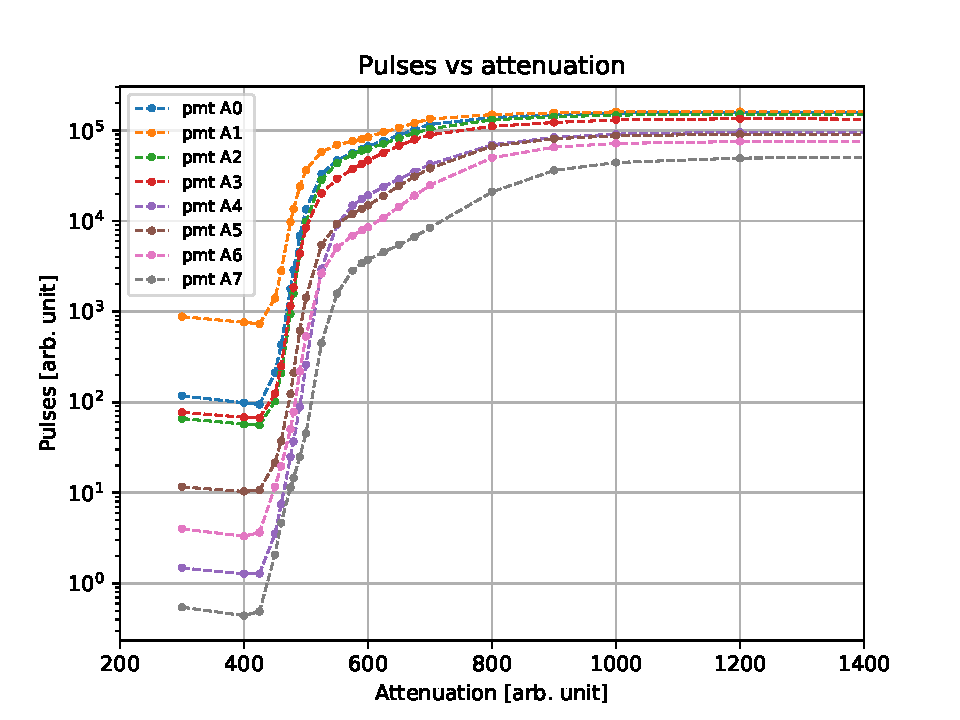
\includegraphics[width = 0.5\textwidth]{Analysis/CalibrationPMT/AttenuationScanA.pdf}}
\end{figure}


From the fit we obtain three valus for the signal Peak, given in attenuaton units.
We can check the idea behind this, visualizing the PMT count in a different way. Because we would like to visualize the number of electrons that generate a certain signal in the detector, we can think of differentiating the data showed in the plot \ref{fig:AttScan}. The differentiation consist in the difference between the Counts at a certain point and the previous one, and dividing by the increment in attenuation:

\begin{align*}
Spectra = \frac{N(att_{i}) - N(att_{i-1})}{att_{i} - att_{i-1}} 
\end{align*}

\begin{figure}[h]
\centering
\subfloat[][\emph{B0} \label{fig:Spectra}]
{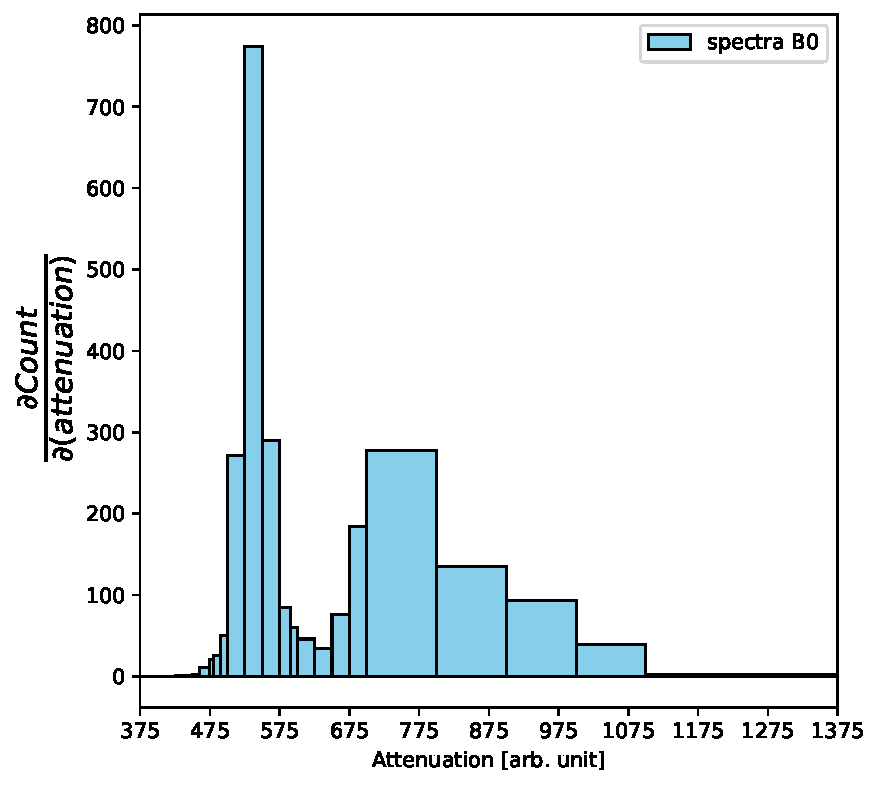
\includegraphics[scale = 0.5]{Analysis/CalibrationPMT/B0.pdf}}
\subfloat[][\emph{B1}]
{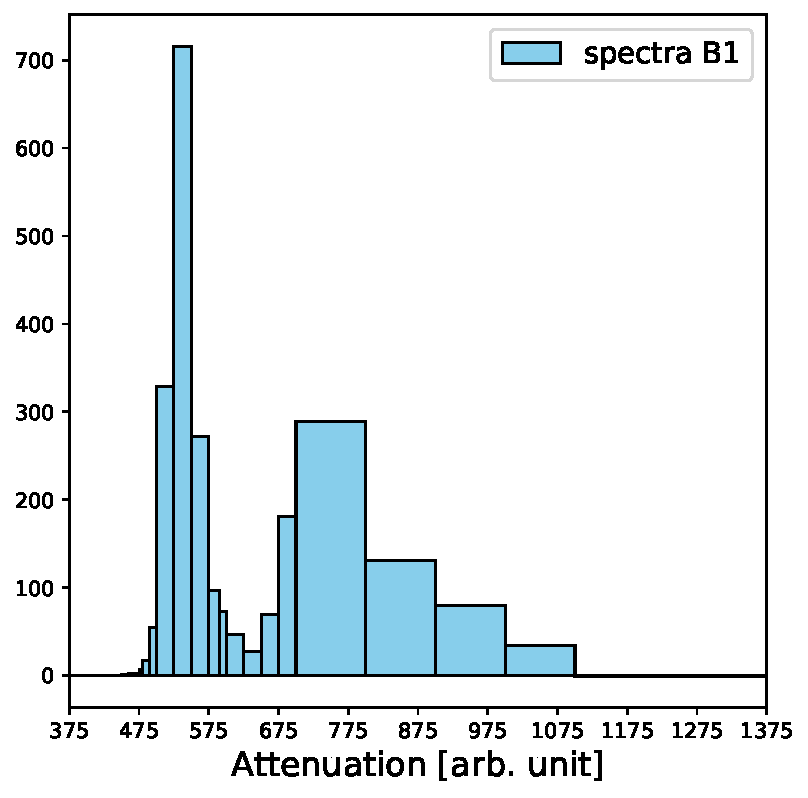
\includegraphics[scale = 0.5]{Analysis/CalibrationPMT/B1.pdf}}\\
\subfloat[][\emph{B2}]
{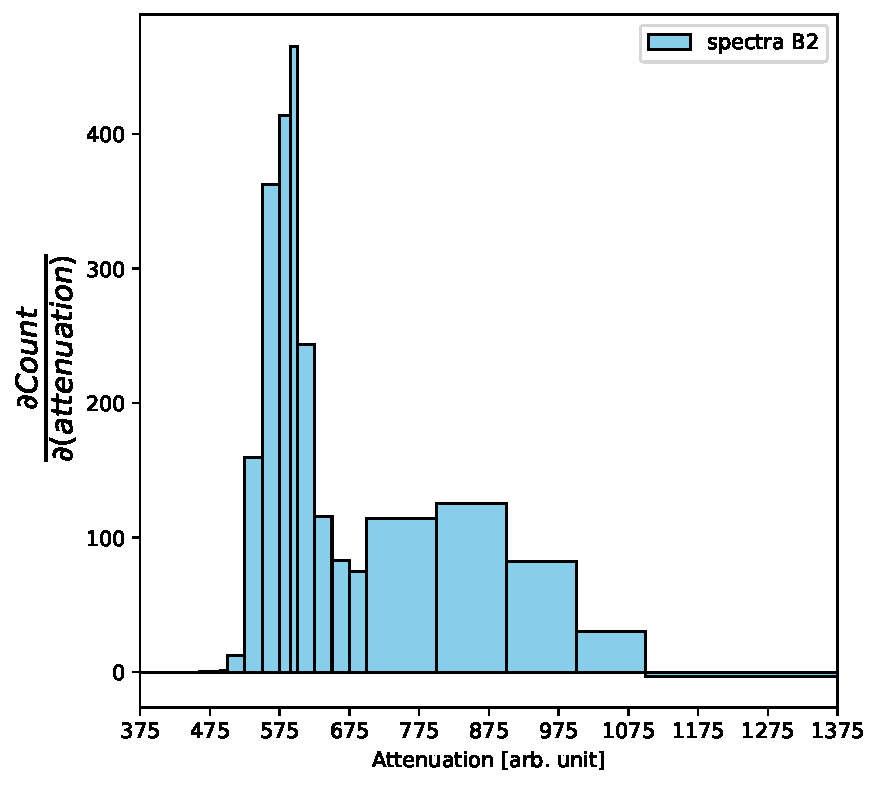
\includegraphics[scale = 0.5]{Analysis/CalibrationPMT/B2.pdf}}
\caption{Reconstructed spectra for Detector B}
\end{figure}

In this way we compute a discrete derivative of the plot showed in \ref{fig:AttScan}, which represent $\frac{\partial N}{\partial att}$. This is, in fact, the spectra of the signal, still given in attenuation units \ref{fig:Spectra}.
This plot are used to identify a good point to select the attenuation values. If we look at the plots \ref{fig:ThrvsAtt}, we can see that the physical threshold does not scale linearly with changing the attenuation value, and for high values of attenuation, the threshold falls quickly at zero. 
Looking at the signal spectra, we identify the first peak as the electron signal. The other peak, for higher attenuation values (on the right), correspond to very low threshold values, and it is identified as the background noise. 
We selected the values of the attenuation between the peaks of the two distributions, maximizing the signal acceptance and trying to reject the background as much as possible.
Our discussion so far is sufficient to carry out the calibration of the PMTs and take data to measure the asymmetry. However, we would like to identify the physical threshold in $\SI{}{\milli \volt}$ instead of attenuation unit. We can use the conversion function that we discussed in \ref{fig:ThrvsAtt}:

\begin{align*}
f(att) = \dfrac{a}{(x - b)^{3} + d}
\end{align*} 

We point out that the parameters of this function have been obtained from data that have not been acquired during this thesis work, moreover the threshold value in the program that controls the NINO board is slightly different (we always used 600, the data are taken with 750), therefore the values in volts need probably to be rescaled by some factor, but for our discussion we are interested in a raw estimation of the signal peak:
With this conversion, we show the same plots in \ref{fig:Spectra}, with the values in the x-axis in $\SI{}{\volt}$ now.

\begin{figure}[h]
\centering
\subfloat[][]{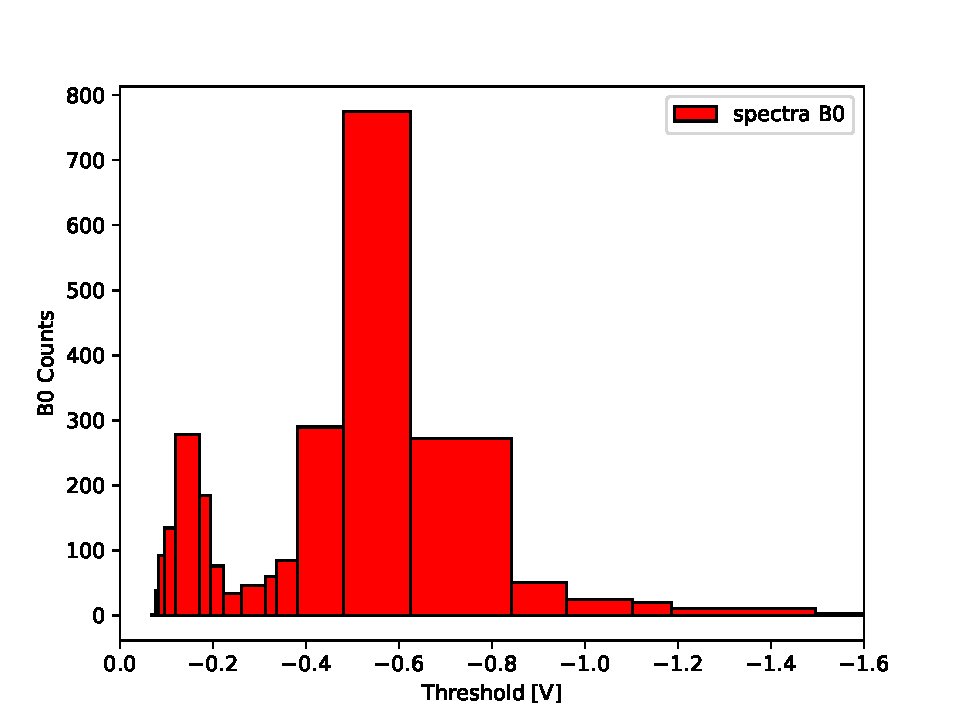
\includegraphics[width = 0.45\textwidth]{Analysis/CalibrationPMT/voltB0.pdf} }
\subfloat[][]{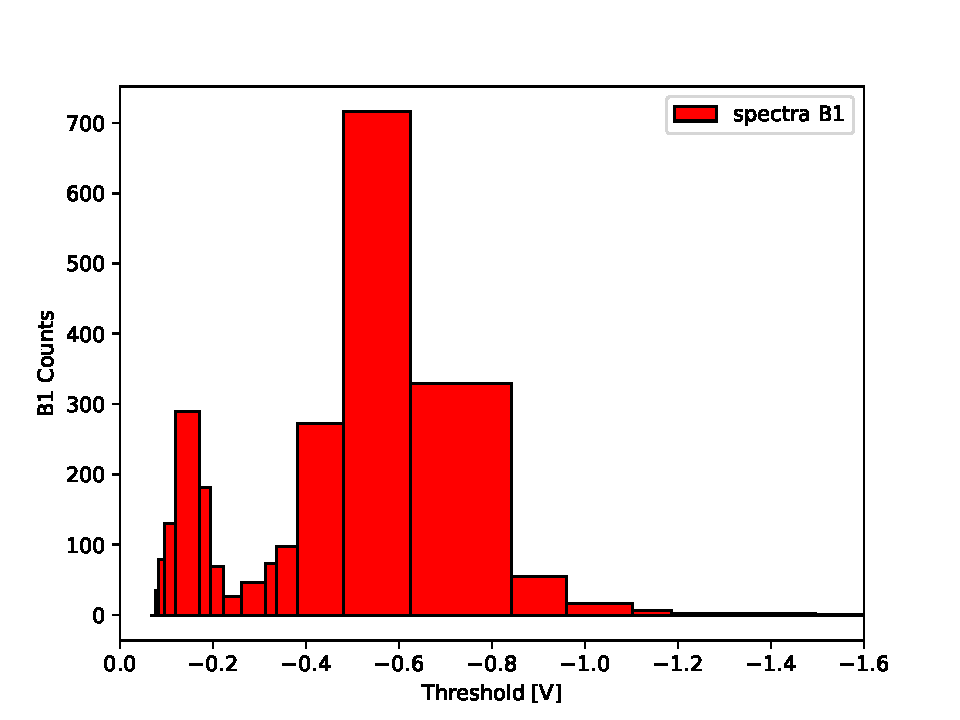
\includegraphics[width = 0.45\textwidth]{Analysis/CalibrationPMT/voltB1.pdf} }\\
\subfloat[][]{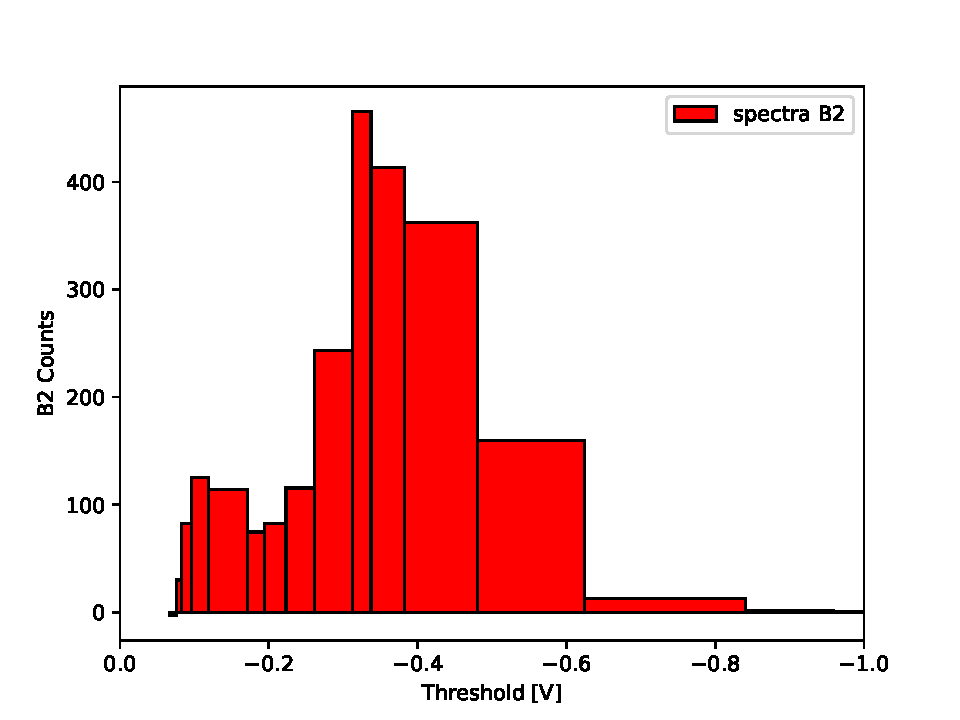
\includegraphics[width = 0.45\textwidth ]{Analysis/CalibrationPMT/voltB2.pdf} }
\end{figure}

We know see clearly two peaks, the signal and the background, that are reversed respect to \ref{fig:Spectra}.

We discuss now a simple model that we used to describe how the PMT Counts vary when we raise the attenuation. From \ref{fig:Spectra}, we assume that the two peaks are described by two gaussian distributions. Now if we think about the the probability for a signal to pass the selection, this quantity is equal to the probability of being in below the attenuation value. Using now the fact that the probability are given by the cumulative of the gaussian distribution (probability of being in the right tail) it is straightforward to deduce:

\begin{align*}
P(signal > thr) = \, \Phi(x) = \dfrac{1 + Erf(\dfrac{x - \mu}{\sqrt{2} \sigma })}{2}
\end{align*}

Considering that we have the sum of two gaussian distribution, we end with:

\begin{equation}
\begin{split}
N(att) = \frac{n_{1} + n_{2}}{2} + (\frac{n_{1}}{2}) Erf(\dfrac{x - \mu_{1}}{\sqrt{2} \sigma_{1} })   + (\frac{n_{2}}{2}) Erf(\dfrac{x - \mu_{2}}{\sqrt{2} \sigma_{2}}) \\
\end{split}
\end{equation}

This model is used to fit the data. The result is shown in the following picture, the parameters obtained from the fit are reported below:

\begin{figure}
\centering
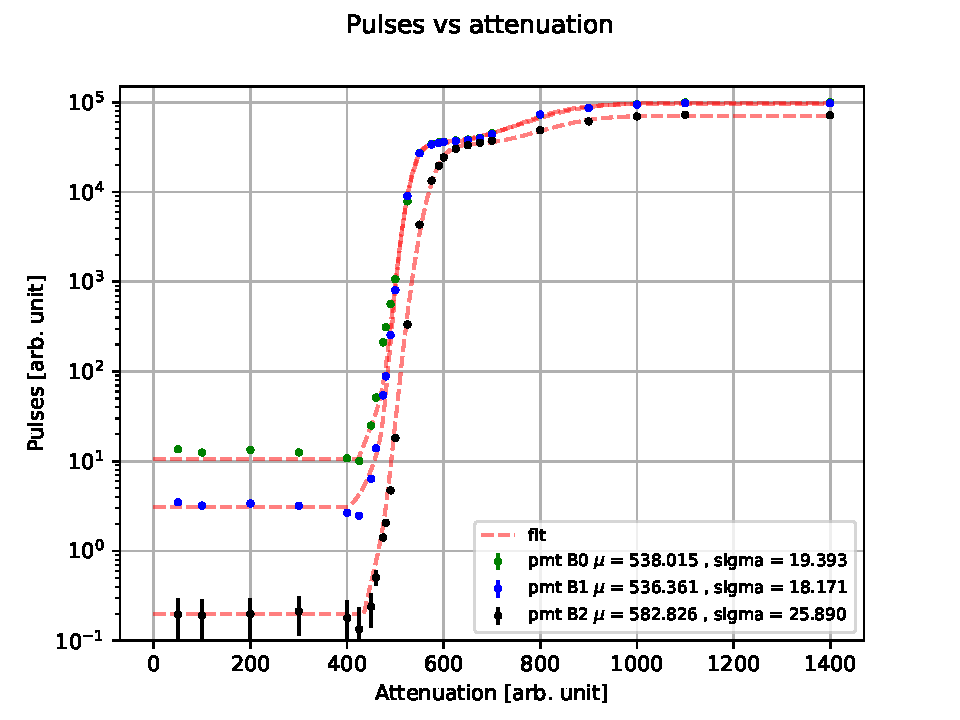
\includegraphics[width = 0.65\textwidth ]{Analysis/CalibrationPMT/Fit_attenuation.pdf}
\end{figure}

\begin{table}
\centering
\begin{tabular}{c|c|c|c|c|c|c}
\hline
 PMT   &  $\mu_{1}$         &  $\sigma_{1}$         & $\mu_{2}$          & $\sigma_{2}$   & n1                & n2                 \\
\hline
 B0    & 538.0 +/- 1.3 & 19.4 +/- 1.1 & 798 +/- 8 & 103 +/- 4 & 34277 +/- 662 & 64244 +/- 1538 \\
 B1    & 536.4 +/- 0.9 & 18.2 +/- 0.7 & 783 +/- 5 & 89 +/- 2  & 34053 +/- 475 & 61636 +/- 1109 \\
 B2    & 582.8 +/- 1.2 & 25.9 +/- 1.0 & 824 +/- 8 & 88 +/- 6  & 32880 +/- 758 & 37930 +/- 1245 \\
\hline
\end{tabular}
\end{table}

From these result we measure the mean $\mu_{1}$ and $\mu_{2}$ for the signal and the background given in attenuation units. The correct value of attenuation is set between the two observed peaks, in order to rejects the background and take only the signal coming from the scattered electrons. The same procedure was followed also for the detector A, the plots are not reported here, for brevity, but in the appendix.

\subsection{Auto-calibration Procedure} \label{Autocalib}

In this section we present the last calibration tecniques needed in the data-process. The autocalibration is a special operation mode of the MAMI accelerator, during which the beam current is made to vary in a controlled way. Through these special runs is possible to obtain again the current scaling factor that we discussed in \ref{CurrentCalibration}. Because the current in varying, it is possible to study the linearity of the PMTs. From a linear fit of the PMTs counts vs. current intensity the angular coefficient and the offset are measured. The offset is particual important because give rise of a possible systematic error that influence the final asymmetry result. It is quite simple to demostrate this, if a relation of the type $N = mI + N_{0} $ holds. Consider the following quantity:

\begin{align*}
\overline{N} = \frac{N_{\uparrow} + N_{\downarrow}}{2}
\end{align*} 

we can express $N_{\uparrow}$ and $N_{\downarrow}$ in this way:

\begin{align*}
N_{\uparrow} = \overline{N} + A_{n}\overline{N} \\
N_{\downarrow} = \overline{N} - A_{n}\overline{N} 
\end{align*}

Now we suppose that $\overline{N}$ is linear dependent on the current in the way we defined above, so:

\begin{align*}
N_{\uparrow} = \overline{N} + A_{n}(mI) + N_{0} \\
N_{\downarrow} = \overline{N} - A_{n}(mI) + N_{0} 
\end{align*}

We are supposing that the offset $N_{0}$, we assume that the present offset does not contribute to the asymmetry, i.e. it is not correlated to the signal of the scattered electrons, but is due to processes of another type, therefore in the previous formulas only the $mI$ counts must be multiplied by the asymmetry $A_{n}$. Therefore if we substitute everything in the definition of the transverse asymmetry:

\begin{equation} \label{eq:Systematic}
A^{'} = \dfrac{N_{\uparrow} - N{\downarrow}}{N_{\uparrow} + N{\downarrow}} = \dfrac{A_{n} (2mI)}{ (2mI) + 2N_{0} } = A_{n} \dfrac{1}{1 + \frac{N_{0}}{mI}}
\end{equation} 

In the last passage we learn that the presence of an offset can decrease the recostructed asymmetry. So it's important to determine quantitatively $N_{0}$ and $m$ in order to be able to take care of this effect. The strategy used is quite simple: every three hours of production data, we asked MAMI to start the autocalibration program. With all the auto-calibration runs, we estimate $N_{0}$ for each PMT, separately. Then All this quantities are saved in a file so that the analysis program can retrieve the parameters and subtract them from the PMT counts. \medskip
In this way every three hours the PMT are corrected, this take care also of the possibility that the the linearity of the PMTs can change after hours of use of the PMTs (for example it can decrease the efficiency).

During the autocalibration, the beam current is raised from $\SI{9}{\micro \ampere}$ to $\SI{11.125}{\micro \ampere}$ in step of $\SI{0.125}{\micro \ampere}$:

\begin{figure}[ht]
\centering
\subfloat[][\emph{Autocalibration: in this plot we have the voltage value of I21 monitor. The current is first stabilized around $\SI{10}{\micro \ampere}$, then it is raised from $\SI{9}{\micro \ampere}$ (the step lower down) to $\SI{11.125}{\micro \ampere}$ in step of $\SI{0.125}{\micro \ampere}$.} \label{fig:Autocalibration}]{
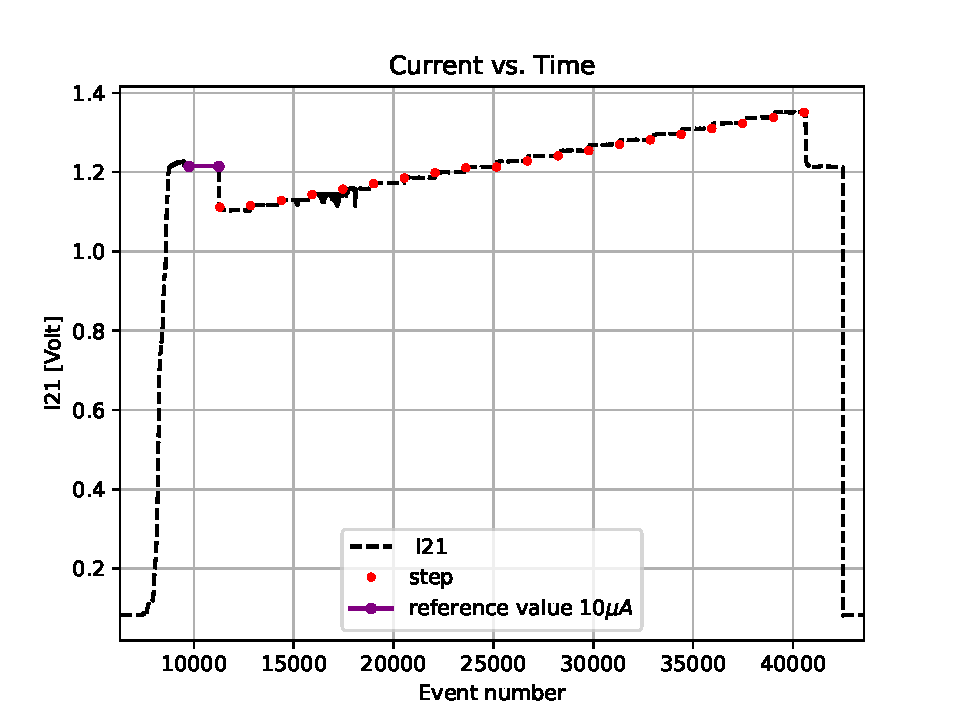
\includegraphics[width = 0.75\textwidth]{Analysis/Autocalib/Current.pdf}}
\end{figure}

With a linear fit we can estimate the scale and the offset to convert from I21 voltage values to physical values of the current. The procedure in repeated for the $8$ autocalibration acquisition we had during the beam time, so we can also take care of possible variations during the time.

\begin{figure}[ht]
\centering
\subfloat[][\emph{Current scan for detector B, the error are multiplied by a factor of $20$.}]{
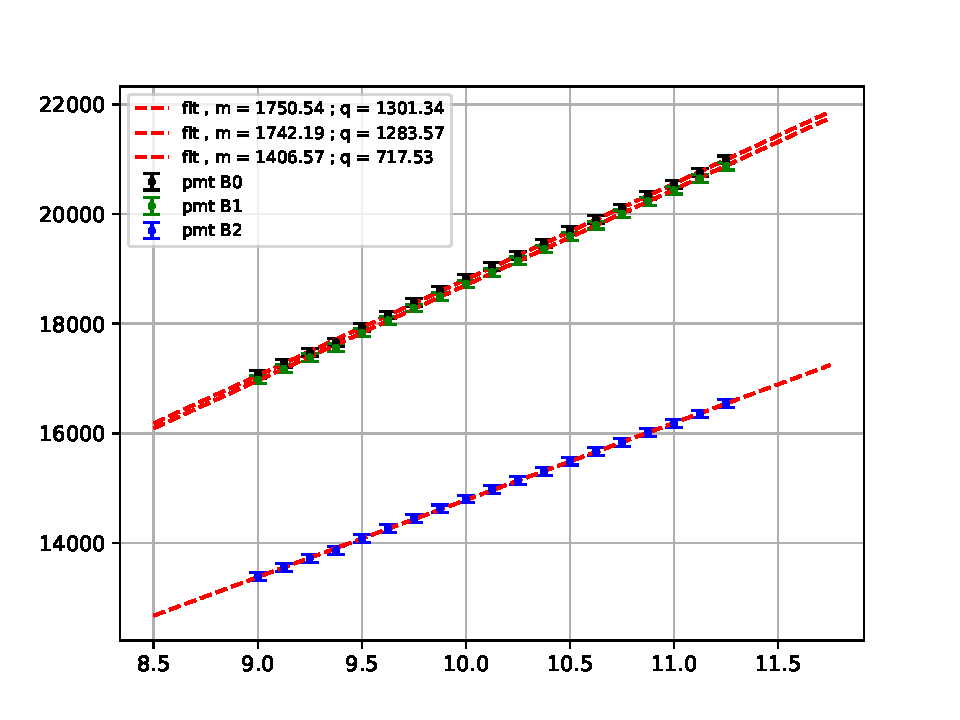
\includegraphics[width = 0.5\textwidth]{Analysis/Autocalib/fitB.pdf}} \\
\end{figure}

\begin{figure}[hbtp]
\centering
\subfloat[][\emph{Current scan for detector A, the error are \\ multiplied by a factor of $20$.}]{
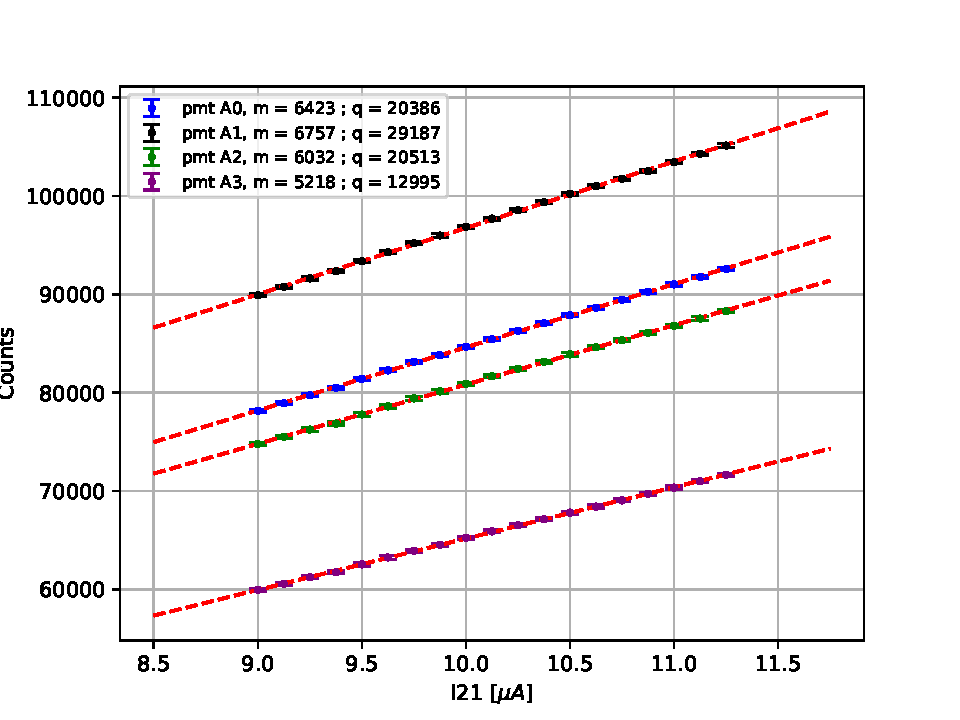
\includegraphics[width = 0.49\textwidth]{Analysis/Autocalib/fitA0-3.pdf}}
\subfloat[][\emph{Current scan for detector A, the error are \\ multiplied by a factor of $20$.}]{
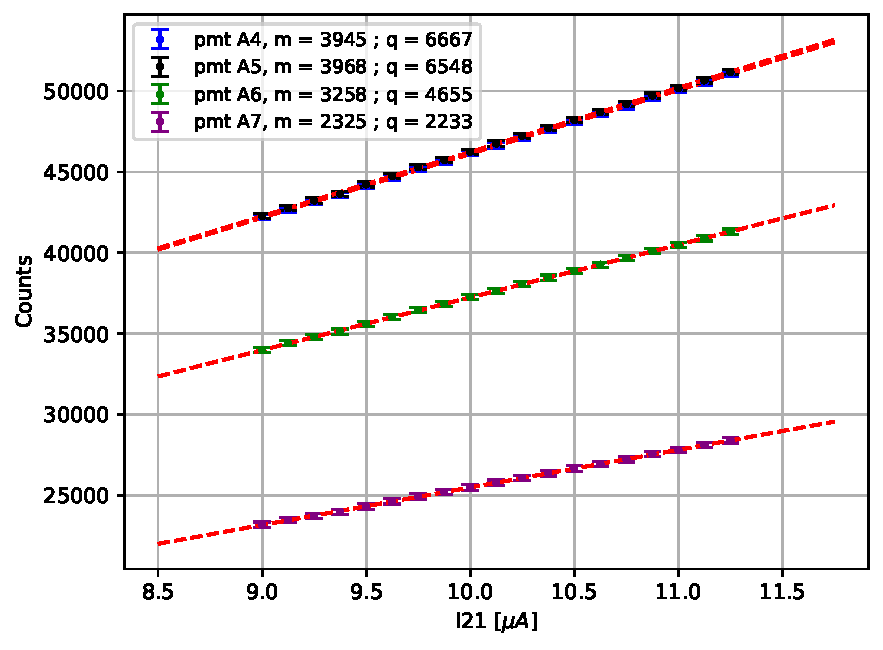
\includegraphics[width = 0.49\textwidth]{Analysis/Autocalib/fitA4-7.pdf}}
\caption{PMT Rates vs current (from I21 monitor), the model used for the fit: $y = mx + q$.}
\end{figure}

\newpage
The figures are referred to the data acquired for the first autocalibration. It's interesting to calculate, from the result of the fit, the factor that appears in \ref{eq:Systematic}:

\begin{table}[ht]
\centering
\begin{tabular}{c|c|c|c}
\hline
 PMT & m [$\SI{}{\micro \ampere}^{-1}$] & Offset & c  \\
\hline
 B0  & 1750 &  1301 &  0.93 \\
 B1  & 1742 &  1283 &  0.93 \\
 B2  & 1406 &   717 &  0.95 \\
 A0  & 6423 & 20385 &  0.75 \\
 A1  & 6756 & 29187 &  0.70 \\
 A2  & 6032 & 20513 &  0.75 \\
 A3  & 5218 & 12995 &  0.80 \\
 A4  & 3945 &  6666 &  0.86 \\
 A5  & 3967 &  6547 &  0.86 \\
 A6  & 3258 &  4655 &  0.87 \\
 A7  & 2325 &  2233 &  0.91 \\
\hline
\end{tabular}
\end{table}
Ignoring the presence of the offset lead two consequences: the recostructed asymmetry is lower, on average $ \simeq 10\%$ less than expected, and the Counts are overstimated. Because the error depend on the PMT counts, as seen in \ref{eq:Error}, this two effect combined add up and worsen the precision and accuracy of the measurement.\\
The result reported in the table can be confronted with the final result that are reported in \ref{result}. 

\newpage



\chapter{Asymmetry on Carbon and Rates on Lead target.}

\paragraph{}
After having described all the calibrations needed, we are ready to analyze the data and measure the \transv from the data collected in second part of the beam time. In this chapter we explain the procedure for the pre-selection of the data (for example the removal of the events with large variation of the beam parameters) and the procedure used to analyze the asymmetry of the two detectors in order to obtain, in the end, a point estimation of $A_{n}$. A section is dedicate to the measurement performed with lead target; through the knowledge of the expected counts per sub-event, we compute the amount of statistics needed to measure the \transv on $Pb$ with an accuracy of $1 ppm$. In the end we discuss the problem of the false asymmetries that can affect the final result, using different method to calculate their contribution.
The amount of data that are available corresponds to 23 hours of acquisitions, that are roughly 1 million of events. 

\section{Rates on Lead}

After all the calibrations are finally perfomed, the experimetal setup is ready to take real "production" data 
to achieve the objectives of the experiment. The first goal of the experiment is to measure the rates on $Pb$ target.
The lead target installed is a made by a thin layer with a thickness of $\SI{0.5}{\milli \meter}$, and it's not isotopically pure. The expected rates are given by the Mott cross section, that we report here \commento{mettere la sezione d'urto Mott, provare a fare i calcoli e vedere se torna}.\medskip

We took $14$ acquisitions lasting $\simeq 2,5$ minutes, which corresponds to $6950$ events. For each of these acquisitions we set the beam current at different values, ranging from $\SI{10}{\micro \ampere}$ to $\SI{22}{\micro \ampere}$ of intesity. The Rates are then reported as a function of the current, a linear model is used to fit the data.

\begin{figure}[hbtp]
\centering
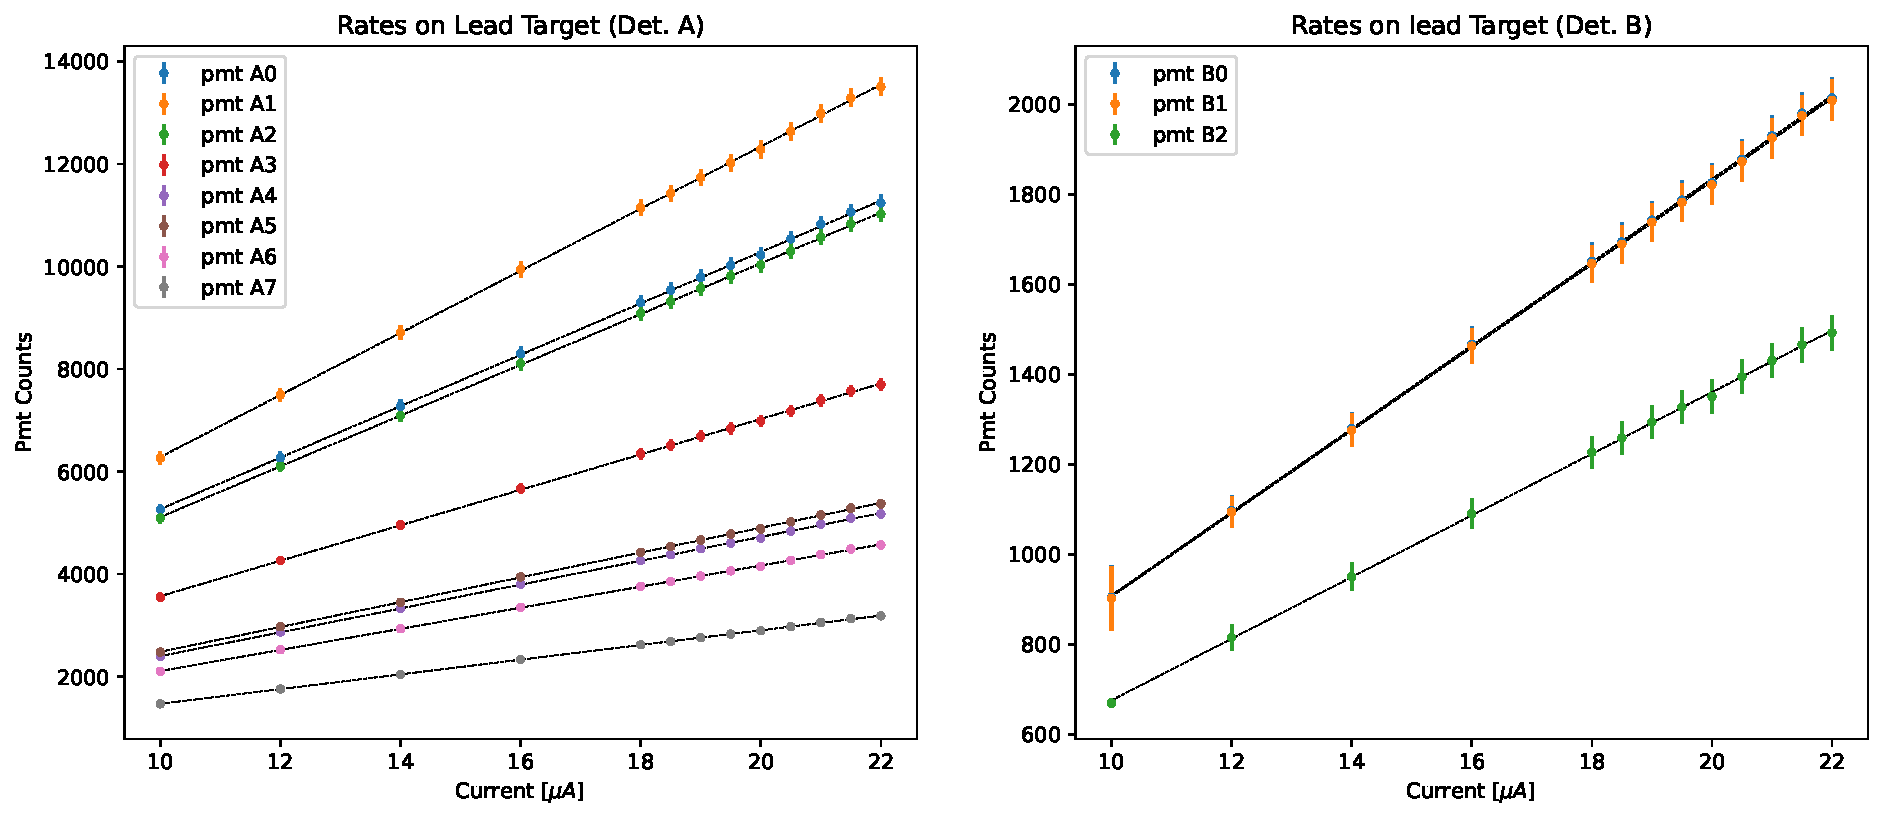
\includegraphics[width = 0.9\textwidth]{Analysis/LeadRates/LeadRates.pdf}
\caption{Rates on lead Target in function of the beam current. The Rates for each PMT of detector A (on the left), and detector B (on the right) are reported.}
\end{figure}

The angular coefficient $m$ and the offset $q$ are reported in the table below. 

\begin{table}[ht]
\centering
\begin{tabular}{lllr}
\hline
 PMT   & m [\SI{}{\micro \ampere}]          & q                &  $\chi^{2}$ (dof = 9) \\
\hline
 A0    & 501.42 +/- 2.17 & 256.55 +/- 39.57 & 13.7521  \\
 A1    & 605.77 +/- 2.31 & 226.11 +/- 42.04 & 13.3783  \\
 A2    & 495.01 +/- 1.47 & 163.04 +/- 26.83 &  6.95713 \\
 A3    & 345.68 +/- 1.6  & 113.4 +/- 29.16  & 12.1727  \\
 A4    & 232.58 +/- 0.9  & 74.38 +/- 16.44  &  5.36892 \\
 A5    & 241.95 +/- 0.74 & 65.79 +/- 13.51  &  3.48398 \\
 A6    & 205.79 +/- 0.65 & 52.38 +/- 11.87  &  3.0892  \\
 A7    & 143.42 +/- 0.47 & 36.49 +/- 8.55   &  2.26341 \\
 B0    & 92.55 +/- 0.34  & -16.88 +/- 6.16  &  2.05286 \\
 B1    & 92.29 +/- 0.33  & -16.9 +/- 5.97   &  1.92163 \\
 B2    & 68.48 +/- 0.32  & -9.34 +/- 5.91   &  2.81988 \\
\hline
\end{tabular}
\end{table}


The PMT Counts with this target, increase from $100$ counts for detector B to $500$ counts every $\SI{1}{\micro \ampere}$.  The experimental error $\sigma$ related to the asymmetry was studied in \commento{aggiungi richiamo}, we recover the formula:

\begin{equation}
\sigma = \sqrt{\dfrac{1}{2 N \cdot n}}
\end{equation}

we remind to the reader that $N$ are the Counts per sub-event, while  $n$ is the number of event analyzed.
Now estimate the amount of statistic needed to measure the asymmetry with some degree of accuracy. Let's suppose that we want to obtain, for each PMT, an error not greater than $4 ppm$. With this accuracy, the asymmetry obtained for detector A will have an error given by $\frac{4ppm}{\sqrt{n_{PMT}}} \simeq 1.5 ppm$.
We computed the time needed to achieve this accuracy for both the two detectors, given in total hours of beam-time. To simplify the calculation, we assumed that every PMT rates of detector A and B are equal to the averaged counts obtained from the plot above.

\begin{table}[ht]
\centering
\begin{tabular}{c|c|c}
\hline
   current I &   T [h] Det A &   T [h] Det B \\
\hline
        10   &       344 &      1487  \\
        12.5 &       277 &      1185   \\
        15   &       232 &      985 \\
        17.5 &       199 &      843 \\
        20   &       175 &      737 \\
\hline
\end{tabular}
\end{table}

As we will see in the next part of this chapter, focused on the asymmetry on carbon target, the amount of time needed to obtain an accuracy of $\simeq 1.5 ppm$ is roughly $15 h$ with $\SI{10}{\micro \ampere}$. The same measurement with lead will need 23 times the statistic accumulated for Carbon. This involves more experimenta difficulties:

\begin{itemize}
\item deterioration of lead target.
\item need to develop a target cooling system.
\item monitor the radioactivity levels in the experimental hall.
\end{itemize}  
 
\section{Model for Fitting the Data} \label{Model}
\commento{Here I have to explain the model used for describing the data, so the problem of the false asymmetry induced by variations in beam position, angle, current and energy.}
\bigskip

One of the problems of the measurement is to take into consideration the various contributions that can change the value of the asymmetry measured by the experimental apparatus. The raw values of the asymmetry can be affected by the variation of the beam parameters during the time. Let's summarize quickly all these effects:
\begin{itemize}
\item the PMTs counts  can depend on the $(x,y)$ impact position of the beam on the target
\item the variations of the incident angles $\theta_{x}$and $\theta_{y}$ on the target.
\item the uncertain associated with the energy of the Beam, a change in the energy associated with the polarization of the beam leads to different rates for the cross section
\item the uncertain associated with the current of the Beam, in particular a change due to the 
efficiency of the source in producing electrons polarized in the two opposite directions
\end{itemize}

All this quantity, which we will indicate in general with $\delta q$ can influence the asymmetry measured by the PMTs, considering also that the expected asymmetry is in the order of ten part per million, and small asymmetry introduced by fluctuations on the beam parameters are not negligible. Correcting directly the false asymmetries that rise from those uncertainties is a tough task, and it's more easy to adopt a different strategy respect to proceed to the analytical/numerical calculation of each of them . Knowing that the beam parameters produced by Mami are quite stable over the time, we can assume that the measured asymmetry are well described by a linear model as the following:

\begin{equation}
A_{tot} = A_{physical} \cdot P + \delta_{I} + A_{x} \delta x + A_{y} \delta y + A_{\theta_{x}} \delta \theta_{x} + A_{\theta_{y}} \delta \theta_{y}+ A_{E} \delta E 
\end{equation}

$A_{physical}$ is the aim of the experiment, $A_{x}$ and $A_{y}$ are the asymmetries induced by the variation of the position of the beam, $A_{\theta_{x}}$ and $A_{\theta_{y}}$ are the asymmetry associated to angles, $A_{E}$ is the asymmetry associated to the beam energy. 
The relevant assumption is that, for small variation of the beam, the false asymmetry are linearly dependent on the Beam uncertainties (that are $\delta x, \delta y, \delta \theta_{x}, \delta \theta_{y}, delta_{E}$), so a first order approximation seems valid.\\
We must clarify now what we mean with $\delta x, \delta y, \delta \theta_{x}, \delta \theta_{y}, delta_{E}$. Resuming the event structure, that we discussed in \ref{FirstDescription}, we have a sequence of 4 different sub-events, with a polarization pattern that is randomly selected between $\uparrow,\downarrow,\downarrow, \uparrow$ and $\downarrow,\uparrow,\uparrow,\downarrow$. During the $\SI{20}{\milli \second}$ of time length of each sub-event, the vfcs make a single measurement of the beam, and the data are saved in the data tree. The task of the analysis program is to use this raw data to calculate the relevant parameters for the analysis. Because we are working with asymmetries, the absolute values of the parameters listed above is not relevant, instead what is relevant are the differences correlated with polarization state of the beam. Assuming this, $\delta x, \delta y, \delta \theta_{x}, \delta \theta_{y}, delta_{E}$ are replaced with :

\begin{equation}
\begin{split}
\delta {x} & = \Bigl(\dfrac{X_{\uparrow}(1) + X_{\uparrow}(2)}{2}\Bigl)  - \Bigl(\dfrac{X_{\downarrow}(1) + X_{\downarrow}(2)}{2}\Bigl)\\
\delta {y} & = \Bigl(\dfrac{Y_{\uparrow}(1) + Y_{\uparrow}(2)}{2}\Bigl)  - \Bigl(\dfrac{Y_{\downarrow}(1) + Y_{\downarrow}(2)}{2}\Bigl)\\
\delta {E} & = \Bigl(\dfrac{E_{\uparrow}(1) + E_{\uparrow}(2)}{2}\Bigl)  - \Bigl(\dfrac{E_{\downarrow}(1) + E_{\downarrow}(2)}{2}\Bigl)\\
\delta {\theta_{x}} & = \Bigl( \dfrac{\theta_{x,\uparrow}(1) + \theta_{x,\uparrow}(2)}{2} \Bigl) - \Bigl(\dfrac{\theta_{x,\downarrow}(1) + \theta_{x,\downarrow}(2)}{2} \Bigl)\\
\delta {\theta_{y}} & = \Bigl( \dfrac{\theta_{y,\uparrow}(1) + \theta_{y,\uparrow}(2)}{2} \Bigl) - \Bigl(\dfrac{\theta_{y,\downarrow}(1) + \theta_{y,\downarrow}(2)}{2} \Bigl)\\ 
\end{split}
\end{equation}

Each $\delta q$ represents the variation of one of the parameters of the beam within an event, so.
One may wonder why the model doesn't contain a parameter $A_{I}$ to describe the false asymmetry due to the current. We can show theoretically that the values of $A_{I}$ is equal to $1$. Starting from the definition of rate $\Gamma$:

\begin{equation}
\Gamma = \frac{dN}{dt} = I_{0} \, \sigma \, \frac{n_{t}}{S}
\end{equation}

where $I_{0}$ is the beam current, $n_{t}$ is the density of the target, and S is the surface of the beam. If we substitute everything in the definition of $A$:

\begin{equation}
A_{I} = \dfrac{\frac{dN_{\uparrow}}{dt} - \frac{dN_{\downarrow}}{dt}}{\frac{dN_{\uparrow}}{dt} + \frac{dN_{\downarrow}}{dt}} = \dfrac{\sigma_{\uparrow} I_{0 \uparrow} - \sigma_{\downarrow} I_{0 \downarrow}}{\sigma_{\uparrow} I_{0 \uparrow} + \sigma_{\downarrow} I_{0 \downarrow}}
\end{equation}

It should be clear now that the current asymmetry $A_{I}$ is equal to 1, and to take care of the contributions of the current we only need to compute $\delta_{I}$: 

\begin{align*}
A_{tot} = A_{n} + \dfrac{I_{0 \uparrow} - I_{0 \downarrow}}{I_{0 \uparrow} + I_{0 \downarrow}} = A_{n} + \delta_{I}
\end{align*}

This is a direct consequence of the fact that the luminosity is proportional to the beam current, so we don't need to add a new parameter to the model.

\section{Data Pre-selection and Fit}

After all the calibration are performed, the analysis program is ready to produce the data-files suitable to analyze the asymmetry data for Carbon. \\
The Data file that are produced from the binary files are simply files in txt format, where the data are stored in columns. Before proceeding with the linear fit, however, it is necessary to visualize the data to check that there are no anomalous behaviors. In fact the data can contain moments of loss of the beam current and sudden interruptions, loss of polarization of the beam and even setting errors by MAMI operators can affect the experiment. Carbon data were taken from November 2nd to 4th, and consist of $28$ runs, each $1$ hour long.
The first step is to observe the PMT counts and the current trend, in order to be able to identify sudden interruptions of the beam, outliers and to check the behaviour. Here we show the trend over time for the series runs: 

\begin{figure}[hbtp]
\centering
\subfloat[][\emph{Counts vs. time, the plot represent the Count trend versus time, made for all the runs acquired during the beam time. The conversion from event number to time is made knowing that each event correspond to $\SI{80}{\milli \second}$. A total of 22 hours of beam was collected.} \label{fig::CountTrend}]{
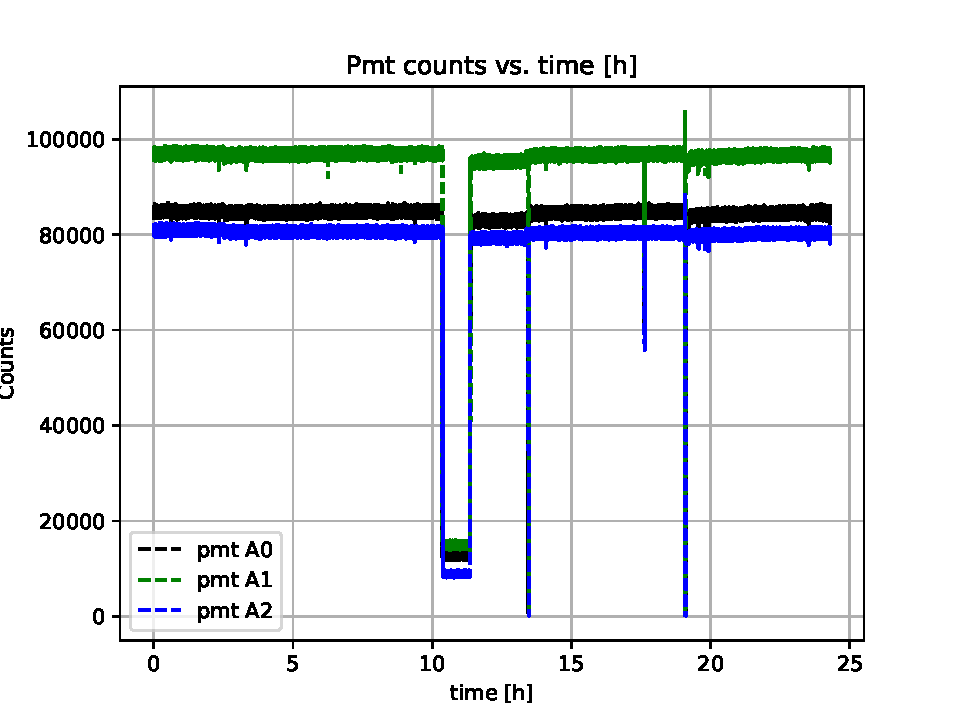
\includegraphics[width = 0.45\textwidth]{Analysis/Dataselection/BeamExample.pdf}}
\subfloat[][\emph{Asymmetry trend for PMT A0} \label{fig::AsymTrend}]{
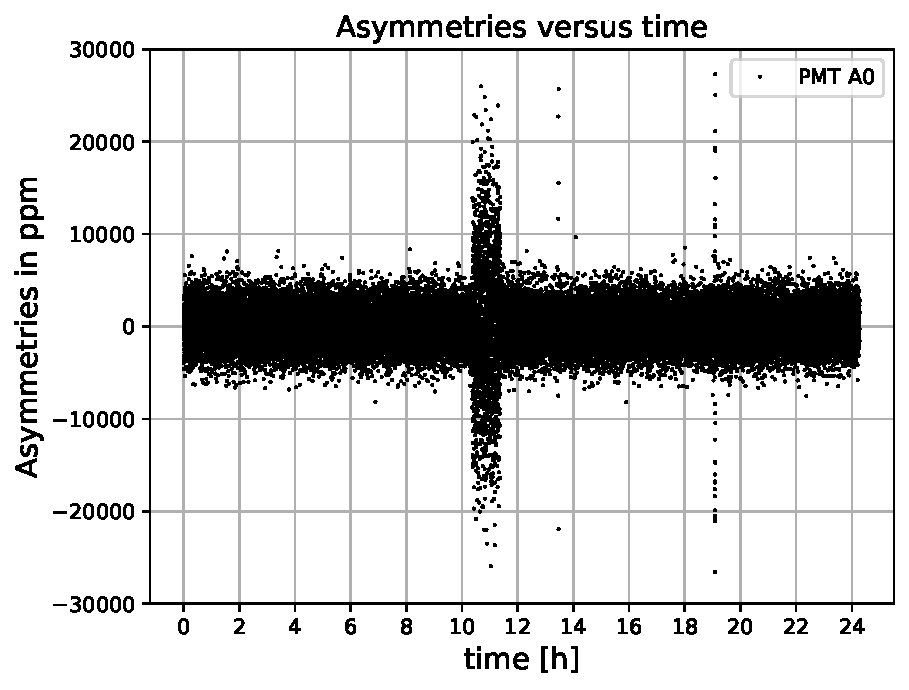
\includegraphics[width = 0.45\textwidth]{Analysis/Dataselection/AsymmetryTrend.pdf}}
\end{figure}

This plot show that after 10 h of data acquisition the PMT counts (\ref{fig::CountTrend}) dropped rapidly. If we show the current trend over the time (\ref{fig::CurrentTrend}) we do not see a corresponding decrease in beam intensity. Also the $x,y$ position (\ref{fig::PositionTrend}) and the energy monitor of the beam do not show a strange behavior, so we reject the possibility that the beam was not properly aligned to the target. \\
We have the strong suspect that this issue come from a failure to be attributed to the NINO board. In fact for all the PMTs, during that time interval, the  counts are equal to the offsets measured with the auto-calibration run. Our suspect is that the threshold and attenuation settings that are loaded during the initialization of the DAQ program were not set correctly. For the analysis, those data are rejected completely.\\
Apart from this, we observe in (\ref{analysis}) sudden variations of the asymmetry around $13.5 h$ and $19 h$, that correspond to decreases in the plot on the left. We reject these data because we observe the same variation also for the current monitor, which means that the beam intensity fall quickly to $0$ for a short period of time. 

\begin{figure}[hbtp]
\centering
\subfloat[][\emph{Current trend over time.} \label{fig::CurrentTrend}]{
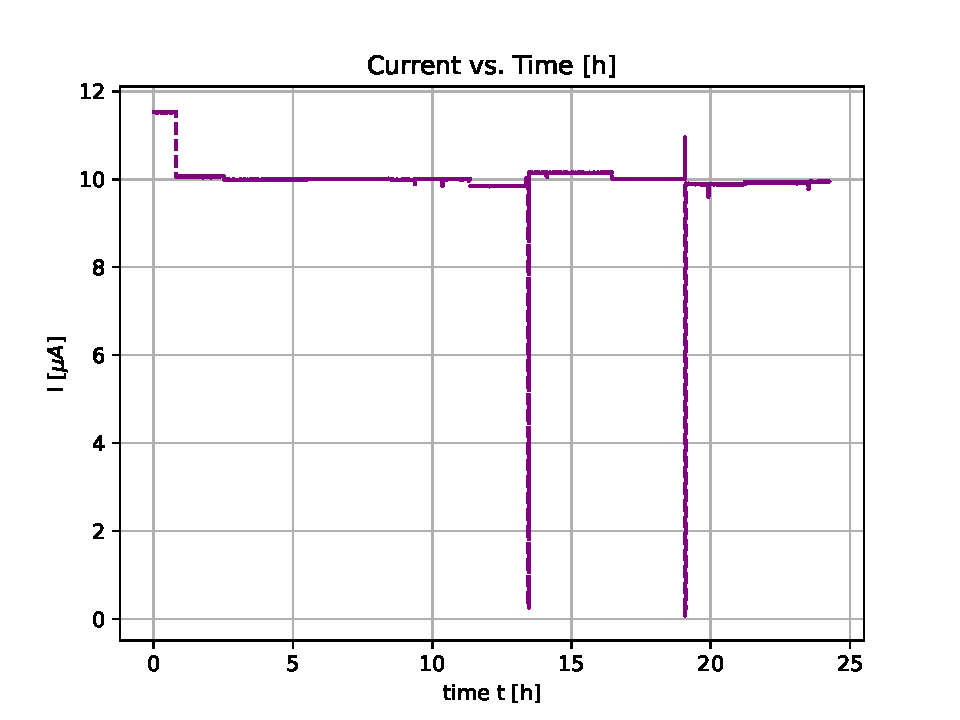
\includegraphics[width = 0.45 \textwidth]{Analysis/Dataselection/CurrentTrend.pdf}}
\subfloat[][\emph{$X,Y$ beam position over time} \label{fig::PositionTrend}]{
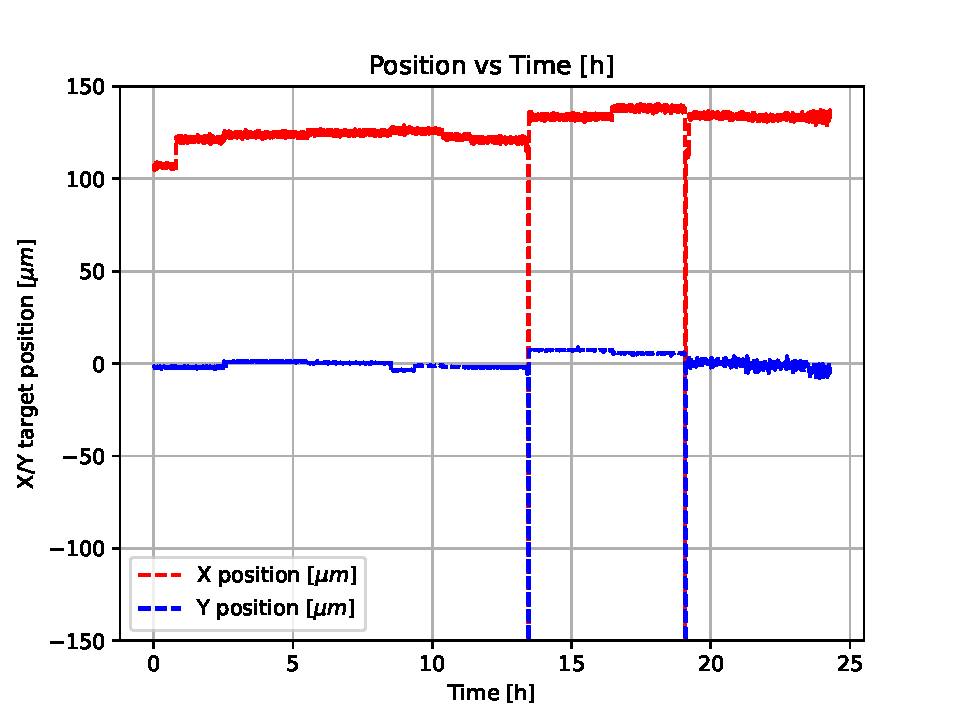
\includegraphics[width = 0.45\textwidth]{Analysis/Dataselection/XYtrend.pdf} }
\end{figure}

Now we focus our attention on the correlated-difference values. We remind the reader that these quantities, that are used as independent variables for the fit, as explained before, are defined as 

\begin{align*}
\delta x =  \frac{(x_{up,1} + x_{up,2})}{2} - \frac{(x_{down,1} + x_{down,2})}{2}
\end{align*}

and are calculated within each single event, to identify the differences with respect to the various quantities such as position, energy... which correspond to different states of polarization.
Several histograms are produced (\ref{fig:IstogrammiParametri}). These plots are useful to quantify the stabilization of the beam: we expect that all the correlated differences are distributed around zero, which implies that there is no systematic difference when the beam has one polarization state respect to the other. The mean $\mu$ and the standard deviation $\sigma$ of the data are reported in the table (\ref{Tab:parametri}) 

\begin{figure}[hbtp]
\centering 
\subfloat[][\emph{$X$ position correlated difference} \label{fig:IstogrammiParametri}]{
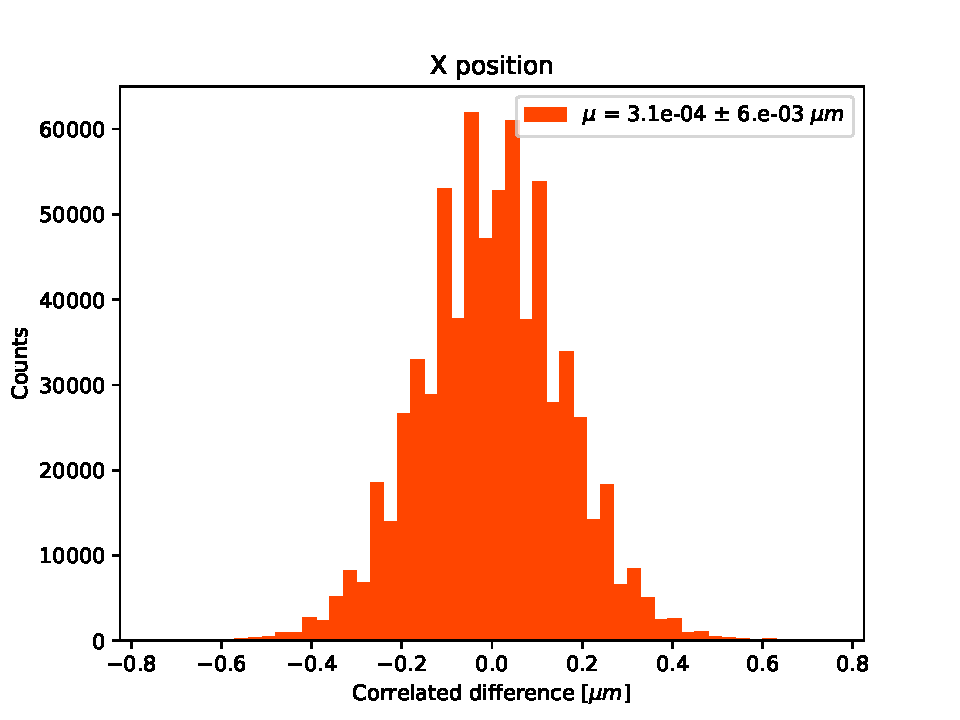
\includegraphics[width = 0.4\textwidth]{Analysis/Dataselection/X.pdf}} 
\subfloat[][\emph{$Y$ position correlated difference}]{
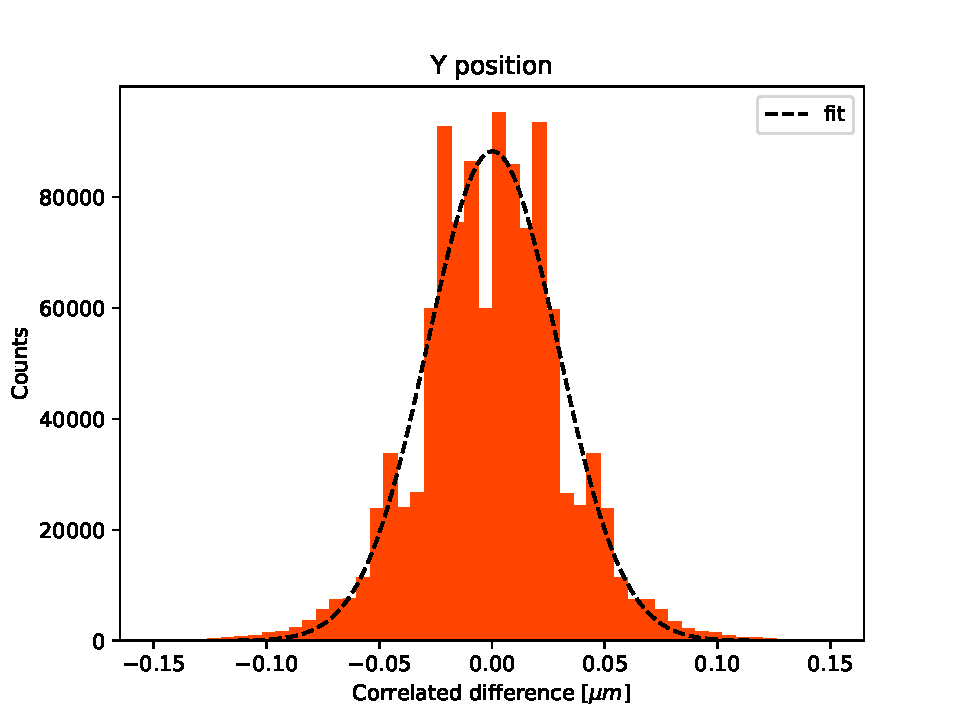
\includegraphics[width = 0.4\textwidth]{Analysis/Dataselection/Y.pdf}}\\
\subfloat[][\emph{$\theta_{x}$ correlated difference}]{
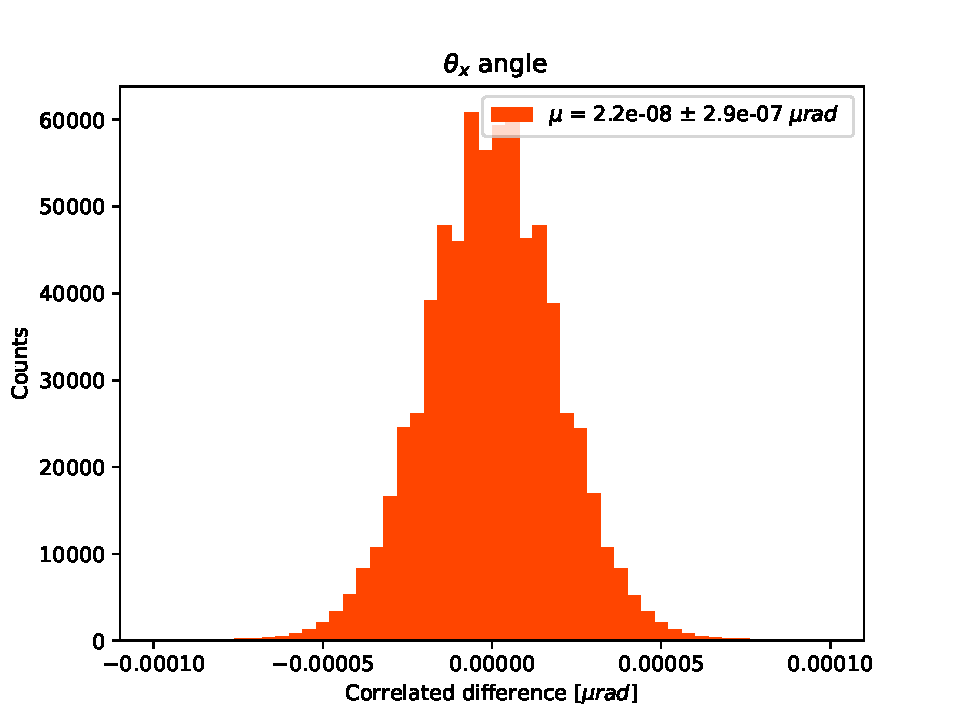
\includegraphics[width = 0.4\textwidth]{Analysis/Dataselection/Xp.pdf}} 
\subfloat[][\emph{$\theta_{y}$ correlated difference}]{
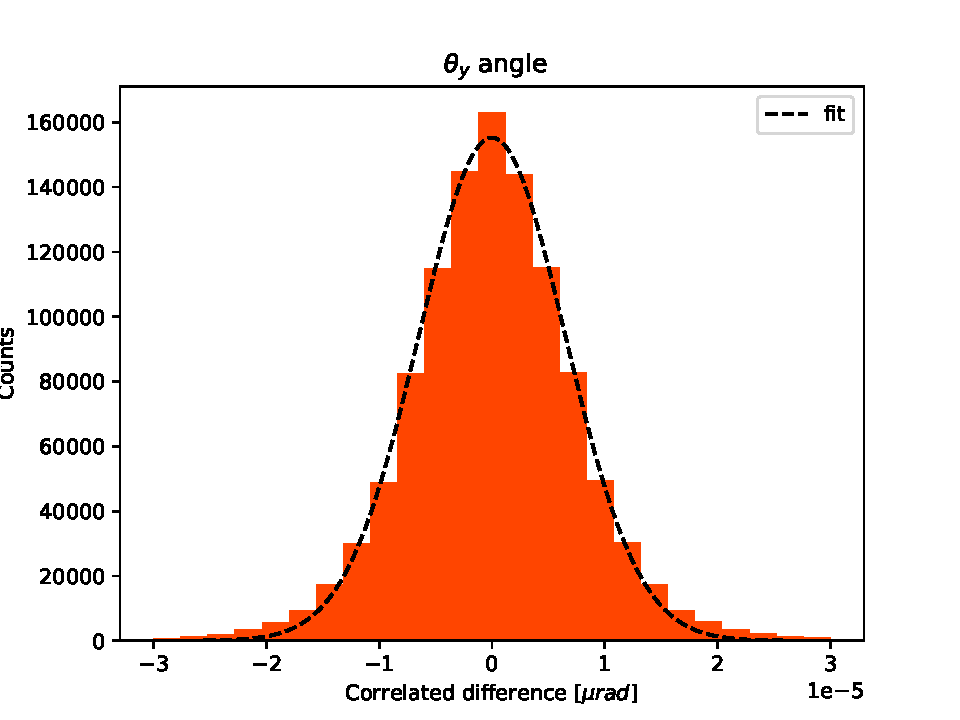
\includegraphics[width = 0.4\textwidth]{Analysis/Dataselection/Yp.pdf}}\\
\subfloat[][\emph{Energy correlated difference}]{
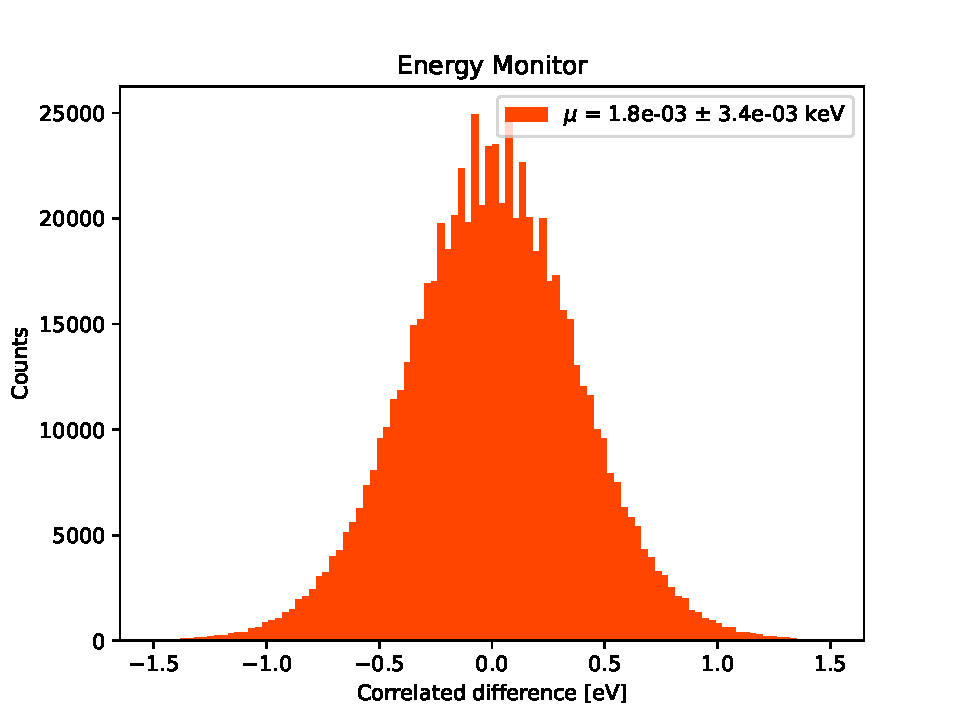
\includegraphics[width = 0.4\textwidth]{Analysis/Dataselection/ENMO.pdf}}
\subfloat[][\emph{Current asymmetry}]{
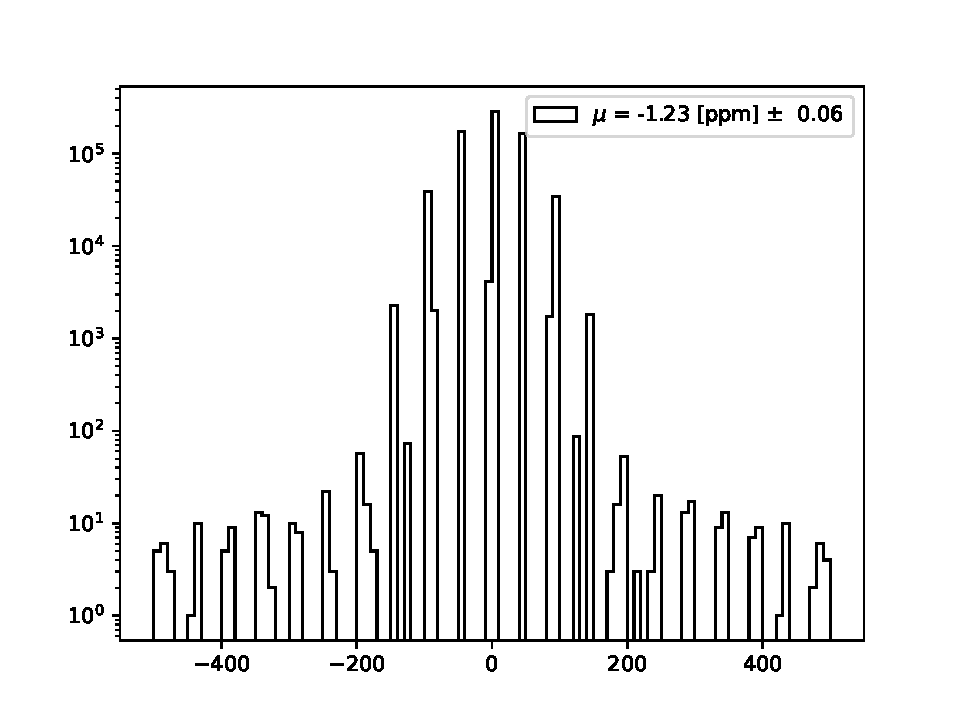
\includegraphics[width = 0.4\textwidth]{Analysis/Dataselection/Current.pdf}}
\end{figure}

Every histogram is generated with $100$ bins. For the current correlated-difference, we find out that the values of the VFCs resistance, which controls $V_{ref}$ value, was set to high. Because of this the precision of the monitor is low, compared to the other, and we observe isolated peaks in the plot. This indicated that for the incoming experiment we have to increase $V_{ref}$ in order to to have a precision comparable to that of other monitors. 


\begin{table}[hbtp]
\centering
\caption{Beam parameters:}
\begin{tabular}{c|c|c|c|c|c|c} 
\hline 
\rule[-1ex]{0pt}{2.5ex} & Beam Parameters: $X [\mu m]$ & $Y[\mu m]$ & $Xp [\mu rad]$ & $Yp [\mu rad]$ & $E [eV]$ & $I [ppm] $ \\ 
\hline 
\rule[-1ex]{0pt}{2.5ex} $\mu$ & $1.31 \cdot 10^{-3}$ & $2.4 \cdot 10^{-4}$ & $3.2 \cdot 10^{-8} $ & $3.6 \cdot 10^{-9}$ & $0.0013$ & $-1.23$ \\ 
\hline 
\rule[-1ex]{0pt}{2.5ex} $sigma$ & $3.7 \cdot 10^{-1}$ & $2.9 \cdot 10^{-2}$ & $ 1.9 \cdot 10^{-5} $ & $6.5 \cdot 10^{-6}$ & $0.38$  & $50.4$ \\ 
\hline 
\end{tabular}
\label{Tab:parametri} 
\end{table}


Looking at the values of the mean and the corresponding error $\sigma$ reported in the plots legend, we observe that mean of $X,Y,\theta_{x},\theta_{y},E$ are compatible with $0$, except for the current correlated-difference, whose values reported already in \textit{ppm} is significantly different from zero. These results are encouraging: we are not able to identify a systematic difference between polarization $+1$ and $-1$. A systematic difference would have produced a value $\mu$ shifted from zero, and a corresponding effect on $A_{n}$. 
With our assumption that the false asymmetries are well described by a linear model, observing that $\mu$ is small and compatible with zero for all the parameters, together with the evidence that $\delta q$ are distributed symmetrical around zero, it could be stated that by averaging the asymmetries:

\begin{align*}
\overline{A} = A_{n} \cdot P + \overline{\delta_{I}} + \overline{\delta_{x}}A_{x} + \overline{\delta_{y}} A_{y} + \overline{\delta_{\theta_{x}}} A_{\theta_{x}} + \overline{\delta_{\theta_{y}}} A_{\theta_{y}} + \overline{\delta_{E}}A_{E} =\\= A_{n} \cdot P + \overline{\delta_{I}} + A_{x}\cdot 0 + A_{y} \cdot 0 +  A_{\theta_{x}} \cdot 0 +  A_{\theta_{y}} \cdot 0 + A_{E} \cdot 0 = A_{n} \cdot P + \overline{\delta_{I}}
\end{align*}  

The contributions related to the false asymmetry should in principle cancel out. We will discuss later, when we will introduce the fit results, whether our assumption reflects the reality. We assume that the false asymmetry that has an effect is $\delta I$: $\overline{\delta I}$ is equal $-1.23 \, ppm$, and we will subtract that to the final result:

\begin{align*}
A_{n} = \overline{A_{tot}} - \overline{\delta I}
\end{align*}

After discussing the removal of the outliers, now will discuss in details the issue regarding the polarization of the Beam. To observe a \transv, it is essential to have a correctly polarized beam.
Unfortunately, we found out that part of the data where acquired with a Beam made by non-polarized electrons. The reason is that during the second night of the beam-time, MAMI operators that controls the quality of the beam switched from polarized beam to non-polarized, unintentionally. These wrong data were acquired during the night of 2nd December and we discovered this problem only the next day. We had no evidence of how many hours of beam were lost. Because this happened during the night, nobody could save the polarization measurement of the beam and identify the runs affected by this problem.
This issue introduces a big systematic error that is potentially decreases the reconstructed $A_{n}$. It is important to identify the runs that share this problem, otherwise the measurements are affected by a bias that is not possible to disentangle from any other systematic effects related to the electronics system of the experiment, therefore also the electronic testing is not possible. 
All the stabilization monitors were active, so the data show apparently the same behaviour of the data with the correct polarization. We can't proceed with an arbitrary cut of the data, because there is the risk to cut off also good data or perform an incomplete removal. The next phase of the analysis is focused on describing a clear method used to identify the data and remove them from the analysis.
 
The procedure to identify the runs with $0\%$ polarization rely to the estimation of the correlation coefficient of the PMTs counts. For every event we have two type of polarization sequence. The polarization $\vec{P}$ of each sub-event is identified with $+1$ and $-1$, that correspond to up and down $\overline{P}$. This values are part of the data tree, and form a sequence $p_{i}$ of the type: $+1-1-1+1$, where i is the index to the i-th sub-events analyzed. If the $\overline{P}$ is different from zero, we expect, due to the \transv, a difference in the number of scattered electrons between sub-events with different $p_{i}$. \medskip

\begin{table}[hbtp]
\centering
\begin{tabular}{|c|c|c|c|c|c|c|c|c|}
\hline 
sub-event & 1 & 2 & 3 & 4 & 5 & 6 & 7 & 8 \\ 
\hline 
Polarity & +1 & -1 & -1 & +1 & +1 & -1 & -1 & +1 \\ 
\hline 
PMT B0 & 101 & 99 & 98 & 102 & 100 & 99 & 97 & 103 \\ 
\hline 
PMT B.. & ... & ... & ... & ... & ... & ... & ... & ... \\ 
\hline
\end{tabular}
\caption{Example of the Polarity sequence and PMT counts that are saved in the analysis program. The values of the PMT counts given are for example. }
\end{table}


This lead to a positive/negative correlation between the sequence $p_{i}$ and the PMT data. In case of $\vec{P} = \vec{0}$, the expected values for the correlation should be zero. \\
We applied this strategy with the hope to identify and remove the block of data with $A_{n} \simeq 0$. The correlation $c$ between the $p_{i}$ and the PMT sequence $N_{i}$ of counts is computed every $t = 1 h$, that correspond to $45000$ events. We plot the averaged correlation for detector A and B, and the correlation of the two detectors together (with the reverse sign for detector B).

\begin{figure}[hbtp]
\centering
\subfloat[][]{
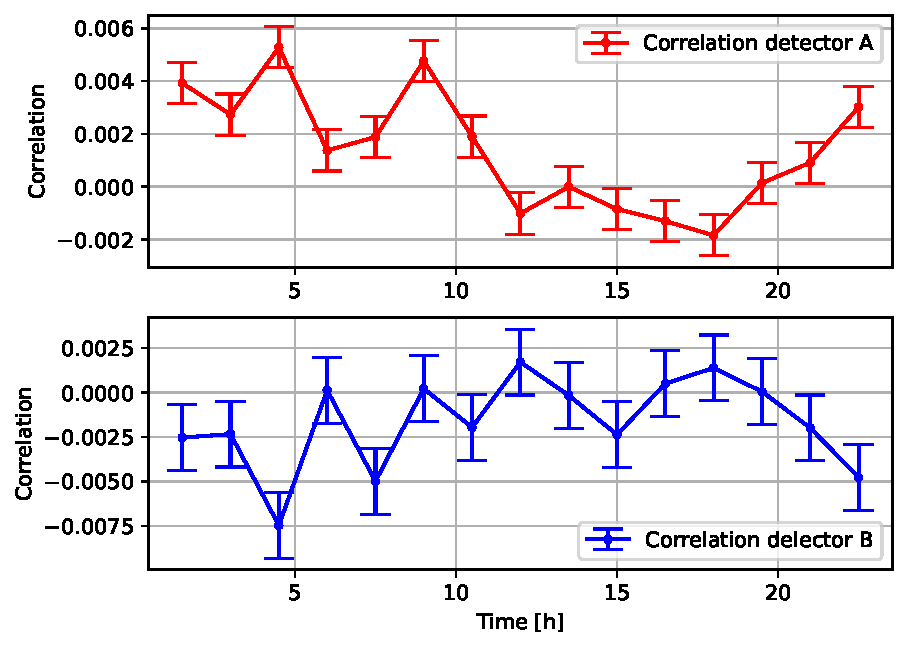
\includegraphics[width = 0.9\textwidth]{Analysis/Dataselection/Correlation.pdf}} \\
\subfloat[][]{
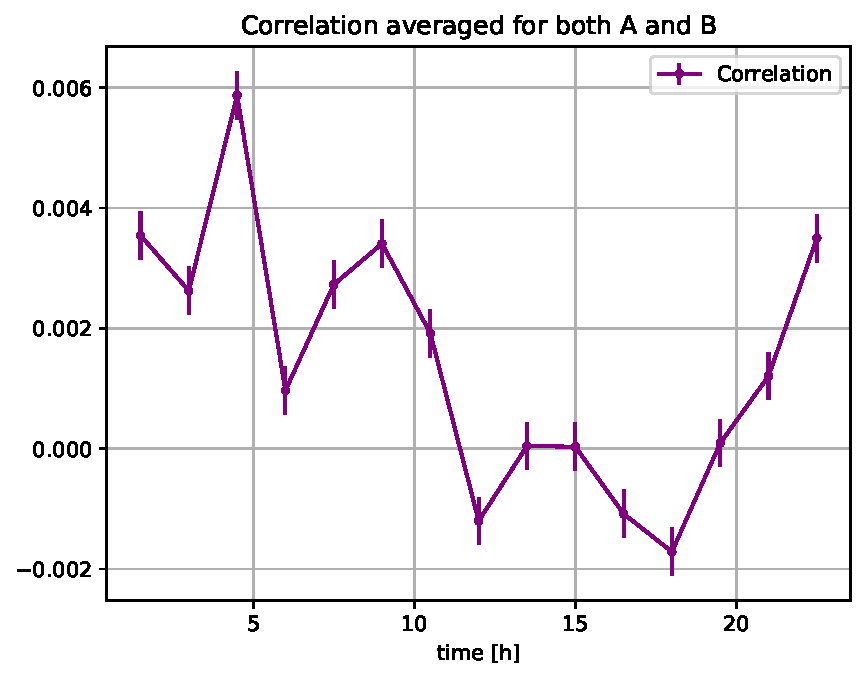
\includegraphics[width = 0.5\textwidth]{Analysis/Dataselection/OverallCorr.pdf}
}
\caption{Plot of the correlation for detector A and on the left, and combining the two detectors results on the right. It's possible to identify a block of run starting at time $t = 12 h$ until $t = 19 h$ where the correlation is small and compatible with $0$. The values can be confronted with the montecarlo, whose error band is in yellow.}
\label{fig:PolarityCheck}
\end{figure}

The correlations coefficient $c$ is clearly dependent on the $\vec{P}$. is we observe that $c$ is compatible with zero, we have an evidence of the block of runs to be removed from the analysis.
The values are reported in figure \ref{fig:PolarityCheck}. The errors for each point are computed with the formula:

\begin{align*}
\sigma_{c} = \sqrt{\dfrac{1 - c^{2}}{N - 2}}
\end{align*} 

The plots show also the expected values for the $c$ computed with a simple simulation, using the values of $A_{n} = 22.5 ppm$ and $P = 0.79$ as an input. The simulation results are obtained following these steps:

\begin{itemize}
\item A sequence of the type $+1,-1,-1,+1$ is generated, long $45000$ events.
\item For each sub-event of the previous sequence, the PMT counts are generated: the counts are sampled from a gaussian distribution with $\mu$ and $\sigma^{2}$ equal to the values measured for both the detectors. To reproduce the correlation with the polarity sequence, the values are shifted accordingly  by a factor $\mu \cdot A_{n} \cdot P$  
\item The previous step is repeated 25 times, and for each iteration we compute and save the correlation between the polarity sequences and the counts.
\item From the values saved, we compute the mean $c$ (the dotted line in plot \ref{fig:PolarityCheck}) and $\sigma_{c}$.
\end{itemize}

Looking at the plots, we observe for detector A a block of runs where $c$ is compatible with 0, in contrast with the values expected from the simulation. Due to the higher error, the corresponding plot for detector B is not clear to interpret, however the plot on the right with the overall results for A and B confirms the evidence for A.
This let us to identify the block of runs that show a behaviour compatible with $\vec{P} = \vec{0}$. It's important to check that validity of this method seeing if the corresponding asymmetry is compatible with $0$ \ref{fig:ZeroAsym}.

\begin{figure}[hbtp]
\centering
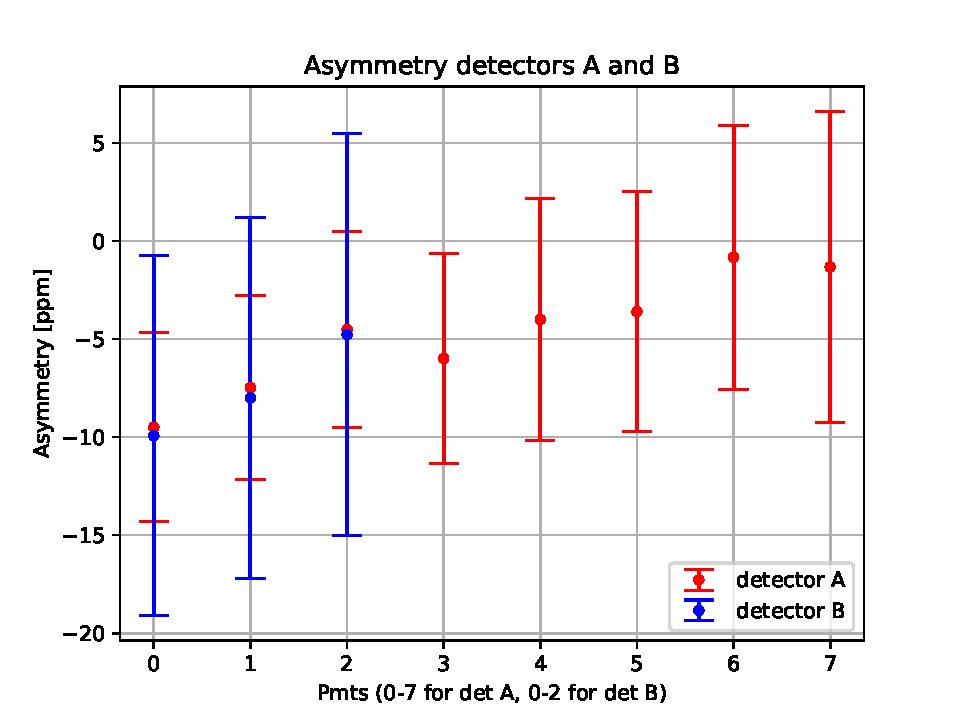
\includegraphics[width= 0.5\textwidth]{Analysis/Dataselection/Nopolarity.pdf}
\caption{Raw-asymmetry computed for the block of runs with $P = 0$. Except for one PMT of detector A, all the values are compatible with $0$ in $1\sigma$.}
\label{fig:ZeroAsym}
\end{figure}

The asymmetry values for this block of runs shows an unexpected behaviour. For both the two detectors we observe negative values. The weighted mean for the two detector is :
\begin{itemize}
\item $A_{B} = -7 \pm 5$ ppm
\item $A_{A} = -5 \pm 2$ ppm
\end{itemize}

The values are not compatible with zero, but are compatible with each other. It is therefore reasonably certain that such data should not be included in the main analysis, because we observe a negative asymmetry for both the two detector is not compatible with the presence of a polarized beam. \\
At this point, it is interesting to study the distribution of the asymmetries measured by the two detectors. Our main assumption is that the asymmetries values are distributed following a normal distribution, around the physical value $A_{n}$. We have produced several histograms to show the PMTs asymmetries. For every histogram we use a gaussian function to fit the data, the reduced $\chi^{2}$ is reported in the table below:

\begin{table}[hbtp]
\centering
\begin{tabular}{c|c}
\hline 
Pmt & reduced $\chi^{2}$ \\ 
\hline
B0 & $1.2 \pm 0.2$ \\ 
B1 & $0.9 \pm 0.2$ \\ 
B2 & $1.23 \pm 0.2$ \\
A0 & $1.2 \pm 0.2$ \\ 
A1 & $0.7 \pm 0.2$ \\ 
A2 & $0.7 \pm 0.2$ \\ 
A3 & $0.9 \pm 0.2$ \\ 
A4 & $1.4 \pm 0.2$ \\ 
A5 & $0.7 \pm 0.2$ \\ 
A6 & $1.1 \pm 0.2$ \\ 
A7 & $1.7 \pm 0.2$ \\ 
\hline 
\end{tabular}
\caption{Reduced $\chi^{2}$ for the gaussian fit of the asymmetry data. The expected value is $1$, the result are generally in agreement with the expected value.  } 
\end{table}

From the values obtained, we don't see a strong evidence to reject our hypothesis. The histograms are reported below:


\begin{figure}[hbtp]
\centering
\subfloat[][]{
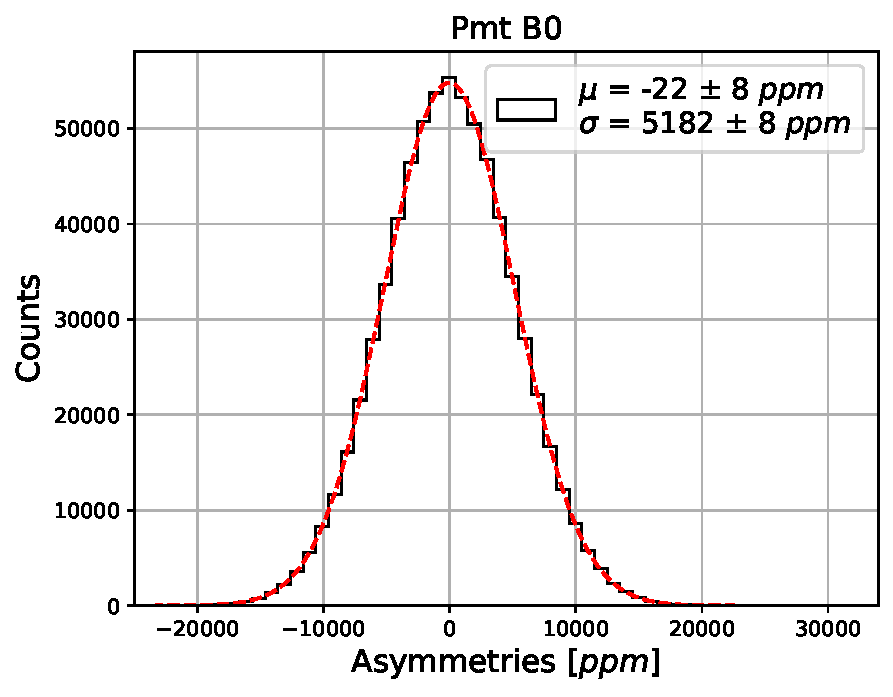
\includegraphics[width = 0.40\textwidth]{Analysis/Histogram/B0.pdf}}
\subfloat[][]{
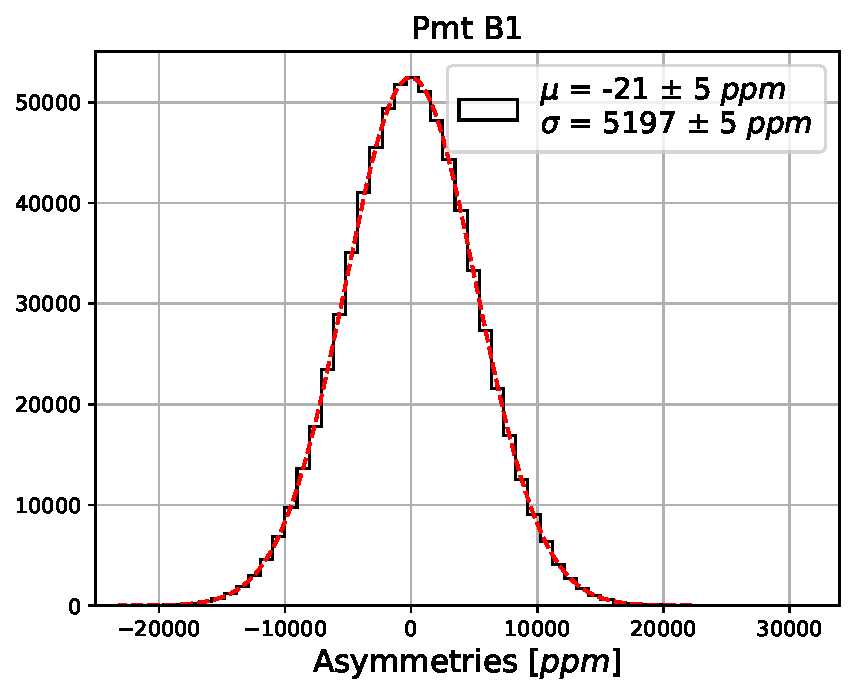
\includegraphics[width = 0.40\textwidth]{Analysis/Histogram/B1.pdf}}\\
\subfloat[][]{
\includegraphics[width = 0.40\textwidth]{Analysis/Histogram/B2.pdf}
}
\caption{Histogram of the Asymmetry for Detector B.}
\end{figure}



We see a good agreement with the hypothesis of normal distributed data . The histograms for detector A are reported below:

\begin{figure}[hbtp]
\centering
\includegraphics[width = 0.40\textwidth]{Analysis/Histogram/A0.pdf} 
\includegraphics[width = 0.40\textwidth]{Analysis/Histogram/A1.pdf}\\
\includegraphics[width = 0.40\textwidth]{Analysis/Histogram/A2.pdf} 
\includegraphics[width = 0.40\textwidth]{Analysis/Histogram/A3.pdf}
\caption{Histogram of the Asymmetry for Detector A.}
\end{figure}

\begin{figure}[hbtp]
\centering
\includegraphics[width = 0.40\textwidth]{Analysis/Histogram/A4.pdf}
\includegraphics[width = 0.40\textwidth]{Analysis/Histogram/A5.pdf}\\
\includegraphics[width = 0.40\textwidth]{Analysis/Histogram/A6.pdf}
\includegraphics[width = 0.40\textwidth]{Analysis/Histogram/A7.pdf}
\caption{Histogram of the Asymmetry for Detector A.}
\end{figure}

\newpage
\newpage
\subsection{Fit with a Linear Model}

To retrieve the asymmetry $A_{n}$ from the data, we assume a linear model where the asymmetries depend on the beam parameters, in the way we discussed before (\ref{Model}). The contributions due to variations of the beam within an events are described with 5 parameters, that are  $A_{x},A_{y},A_{\theta_{x}},A_{\theta_{y}},A_{E}$.
The data are analyzed both using python libraries, and with a fit program implemented in the framework of this thesis. To analyze the data with python, it is used the \textit{curvefit} function implemented in the python library \textit{scipy}.
The fit program implements a well know algorithm used in linear regression: the ordinary least square algorithm (OLS).
The OLS algorithm is basic algorithm, the easiest to implement and robust. It relies on few important hypothesis about the characteristics of the data. In principle we could handle all the analysis relying entirely on python. The decision to implements a fit program by ourself is due to the fact that in this way we interface directly to the analysis program, that is written in \textit{c++} code. 
the assumption underlying linear regression is that there is a relation between the data of this type:

\begin{equation}
 y \, = \, \vec{x} \cdot \vec{\beta} + \epsilon
\end{equation}

$\vec{x}$ are the independent variables, $\vec{\beta}$ are the parameters and $\epsilon$ is a noise, that is supposed to be gaussian distributed (however, the robustness of the OLS algorithm let to relax this request). Another important assumption is that the linear variables are not correlated. 
This last request is particularly important, as related data cannot be processed with either of the two algorithms used.
Before proceeding with the fit, it is necessary to verify this assumption. \medskip
The first step so is to compute the correlation matrix for the beam parameters, we report in a table the values obtained:

\begin{table}[hbtp]
\centering
\begin{tabular}{|c|c|c|c|c|c|c}
\hline 
             & $X$ & $Y$ & $\theta_{x}$ & $\theta_{y}$ & $E$ & $I$\\ 
\hline 
$X$            & 1 & -0.02 & -0.99 & 0.06 & 0.04  & -0.03\\ 
\hline 
$Y$            & -0.02 & 1 & 0.01 & -0.65 & 0.01  & -0.02\\ 
\hline 
$\theta_{x}$ & -0.99 & 0.006 & 1  & -0.005 & -0.05 & 0.03\\ 
\hline 
$\theta_{y}$ & 0.06 & -0.65 & -0.05 & 1 & -0.003  & 0.03\\ 
\hline 
$E$            & 0.04 & 0.005 & -0.05  & -0.003  & 1 & 0.26\\ 
\hline 
$I$            & -0.03 & -0.02 & 0.03  & 0.03 & 0.26 & 1\\ 
\hline
\end{tabular} 
\end{table}

It's immediate to observe that for $(\theta_{x},X);(\theta_{y},Y)$ the values for the correlation are high compared to the other parameters. 

\begin{figure}[hbtp]
\centering
\subfloat[][\emph{}]{
\includegraphics[width = 0.45 \textwidth]{Analysis/Fit/X_Xp.pdf} }
\subfloat[][\emph{}]{
\includegraphics[width = 0.45 \textwidth]{Analysis/Fit/Y_Yp.pdf}}\\
\subfloat[][\emph{}]{
\includegraphics[width = 0.45 \textwidth]{Analysis/Fit/Y_X.pdf}}
\end{figure}

The plots confirm the linear dependence between those parameters. With this evidence, it's clear that the have to modify the model to fit the data. We decided to include as linear independent variables only : $I,X,Y,E$.

Before proceeding with the fit, it's interesting to study how $A_{n}$ evolves with the increase of the data. What we intend is to plot the averaged values $\overline{A_{n}}$ as the number of data increases, where the average is made on all data collected from time $t = 0$ up to time $t = t_{1}$ (\ref{fig:AsymOverTime}). 

\begin{figure}[hbtp]
\centering

\subfloat[][\emph{Averaged asymmetries for each PMT.}]{
\includegraphics[width = 0.45 \textwidth]{Analysis/Dataselection/AveragedAsymmetry.pdf}}
\subfloat[][\emph{Averaged asymmetry for detector A and B. The dotted line correspond to $1\sigma$ error.}]
{\includegraphics[width = 0.45 \textwidth]{Analysis/Dataselection/AveragedAsymmetry2.pdf}}
\caption{Plot of the Asymmetry versus time. The plot show the average over all the events collected from $t = 0$ to $t = t_{1}$. Each line represents $A_{n}$ measured for  PMT (in \textcolor{blue}{blue} detector B and in \textcolor{red}{red} detector A). The values are corrected for the beam polarization, multiplying by $\frac{1}{p}$. No further correction is applied.}
\label{fig:AsymOverTime}
\end{figure}

These plots are useful to check that the asymmetries converge to a certain value, and that there are no steepy variations that could be related to the presence of remaining outliers. Besides this we observe that the sign of the asymmetries for the two detectors are opposite, in agreement with what we expect from the different kinematic. In fact the sign of the asymmetry is given by the sign of the cross product $\vec{k} \times \vec{k}'$. For detector A the cross product has a positive module, while for the detector B it is negative.
For a better visualization of the data, especially to observe the dependence of the asymmetry on the Beam parameters measured, it is useful to plot $A$ versus each of the beam parameters. Unfortunately, the statistical error associated to the asymmetry is too high to appreciate whether there is a linear dependence in the data. For example here we plot the asymmetries $A$ versus $X$.

\begin{figure}[hbtp]
\centering
\includegraphics[width = 0.5\textwidth]{Analysis/Fit/A_vs_X.pdf}
\caption{PMT A0 asymmetries versus X beam position. Because of the statistical uncertainties, it is not possible to visualize a linear dependence in the data.}
\end{figure}

The statistical error associated to $A$ is too high to identify a trend in the values. A different approach is to divide the $X$ axis in small interval, like the procedure of binning, and average all the asymmetries that fall in the same interval. This reduce the amount of data, but decrease the statistical fluctuations. For a plot of this type each point represents the overall asymmetry for a particular interval of $X$ ,$Y$ and $E$.
 
\begin{figure}[hbtp]
\centering
\subfloat[][]{ 	\includegraphics[width = 0.45\textwidth]{Analysis/Fit/pmtA0_X.pdf}}
\subfloat[][]{ 	\includegraphics[width = 0.45\textwidth]{Analysis/Fit/pmtA0_Y.pdf}}\\
\subfloat[][]{ 	\includegraphics[width = 0.5\textwidth]{Analysis/Fit/pmtA0_E.pdf}}
\caption{ $A$ versus $\delta x$, $\delta y$ and $\delta E$. The plot are generated with 50 equally spaced bins. The red line is the best fit with a linear model.}
\end{figure} 

We report for brevity only the values for pmt A0 of detector A. In this case is is more simple to identify the presence of a linear dependence in the data. 
The errors are computed with the formula defined in equation \ref{eq:Error}, considering each interval separately.
Another approach that we can use to further reduce the fluctuations due to the high statistical error of $A_{n}$ is to do an additional average for all the PMTs of each detector. This procedure decrease the error of a factor $\sqrt{8}$ for detector A and $\sqrt{3}$ for detector B. However, this procedure doesn't take care of the different linear dependencies on the beam parameters for the various PMTs considered, so this last procedure is not immune from a possible bias. 

\begin{figure}[hbtp]
\centering
\subfloat[][\emph{ $A$ versus $\delta x$, the linear model is the red line, the second used to fit the data is a polynomial, represented in blue.}]{ \includegraphics[width = 0.5\textwidth]{Analysis/Fit/Xfit.pdf}}
\subfloat[][]{ \includegraphics[width = 0.5\textwidth]{Analysis/Fit/Yfit.pdf}}\\
\subfloat[][]{ \includegraphics[width = 0.5\textwidth]{Analysis/Fit/Efit.pdf}}
\end{figure}

For the $X$ and $Y$ positions, Two models are used to fit the data. The first one is the linear model: 

\begin{equation}
A = m \, \delta x + A_{phys}
\end{equation}

For the second model, we decided to use the following polynomial:

\begin{equation}
A = c \, \delta x^{5} + m \, \delta x + A_{phys}
\end{equation}

For the energy monitor, we have:
\begin{equation}
A = c \, \delta E^{3} + m \, \delta E + A_{phys}
\end{equation}

This choice is due to the fact that we observe that $A$ increases near the tails of the plot, the odd exponent is due to the fact that $A$ has a different sign, positive for left and negative for right.

The values of the fit are reported in the plots. The $\chi^{2}$ of the fit are reported here

\begin{table}[h]
\centering
\begin{tabular}{|c|c|c|c|}
\hline 
detector A & $X$ & $Y$ & $E$ \\ 
\hline 
linear fit $\chi^{2}_{17}$ & 99 & 59 & 94 \\ 
\hline 
alternative model $\chi^{2}_{16}$ & 76 & 55 & 78 \\ 
\hline 
\end{tabular} 
\end{table}

The $\chi^{2}$ values are higher that the expected and we observe that the values for the model 2 are lower than the ones of linear fit.
This high values can be explained with two considerations: the first one is that this procedure of averaging the data based on $x$ interval leads to the loss of information that can influence the fit, the second consideration is that we are ignoring the possible error in the determination of $\delta x$.
Despite this, we observe that using a model with more complicated dependencies doesn't change  the values of $A_{phys}$. Because of this we don't see a strong evidence to change the linear model: 

\begin{equation}
A_{tot} = A_{phy} \cdot P + \delta_{I} + A_{x} \delta x + A_{y} \delta y + A_{E} \delta E 
\end{equation}

\commento{
\begin{equation} \label{eq:ComplicatedModel}
A_{tot} = A_{phy} \cdot P + \delta_{I} + A_{x} \delta x + A_{y} \delta y + A_{E} \delta E + c_{x} \, \delta x^{5} + c_{y} \, \delta y^{5} + c_{E} \, \delta E ^{3}
\end{equation}}

the result of the fit are reported in \ref{tb:resultA}, together with the final result of the asymmetry for detector A and B.

\section{False Asymmetries}
\commento{Seems that is possible to obtain rough estimates of the beam related asymmetries with the results from the fit. For Energy and position it's achievable, while for the angle it's quite hard (in principle sounds possible to perform an analytic calculation of the asymmetry related to the incident beam angle, however Anselm told me that quite often those results are not in agreement with the observed even in the sign!).}

Until now the values for the false asymmetries were threated as the parameters of the fit. In this section we will investigate how we can obtain another different estimations, useful to check the validity of all the process of analysis of the data.

For $\frac{dA}{dX}$ and $\frac{dA}{dY}$, we conceptually exploit the possibility of varying the position of the beam on the target, as we did during one of the calibration phases. Using the same \textit{wobbler 16} we asked MAMI to slowly change the beam position on the X and Y monitor. The change in position has the effect to modify the rates for the two detector, and from them it's possible to extract estimate the two false asymmetries related to the beam position. Now we will see how the two quantities are related.
From the plot \ref{fig:SlowPosition} we see that the counts are scaling linearly with the beam position, so we assume that the $N$ are given by

\begin{align*}
N(x,...) = N_{0} + m \cdot (x - x_{0})
\end{align*}

it is clear that the linear model can't be always good, at some point the electron will be deflected completely out of the detector, and so the counts will fall rapidly to zero. However, the magnets used to deflect the beam are producing small variation in the position, on the order of hundredths of a millimeters.
Let's suppose that the beam position for two sub-events is $x_{1}$ and $x_{2}$, we can calculate the asymmetry between the two event, taking care of the possible effects due to the different position. We write explicitly: 

\begin{equation}
\begin{split}
Asym = \dfrac{N(x_{1}) - N(x_{2})}{N(x_{1}) + N(x_{2})} = \dfrac{N_{0} + m \cdot (x_{1} - x_{0}) - N_{0} - m \cdot (x_{2} - x_{0})}{N(x_{1}) + N(x_{2})} =  \dfrac{m}{2 N_{0} + m \cdot (x_{1} +  x_{2}) - 2m x_{0}}(x_{1} -  x_{2})
\end{split}
\end{equation}

In this equation three different parameters appear: $N_{0}$ is the offset of the linear model, $m$ is the angular coefficient, or the slope, and $x_{0}$ is the initial position respect to we compute the position variation. The first two terms are obtained by a linear fit, while $x_{0}$ is fixed conveniently.

\begin{figure}[hbtp]
\centering
\subfloat[][\emph{Plot for slow variation in $x$ direction for detector B.}]
{\includegraphics[scale=0.5]{Analysis/slowxVariation.pdf}}
\subfloat[][\emph{Plot for slow variation in $x$ direction for detector B.}]{\includegraphics[scale=0.5]{Analysis/slowyVariation.pdf}}
\caption{Plot of the pmt occurrences versus the $X$ position. The $X$ position was slowly changed during this acquisition.}
\label{fig:SlowPosition}
\end{figure}


We can approximate the denominator deleting the term $ m \cdot (x_{1} +  x_{2})$ which should be equal, at first order, to $- 2m x_{0}$, and should cancel out. We end with:

\begin{equation}
Asym = \dfrac{m}{2N_{0}}(x_{1} -  x_{2})
\end{equation}

The term in front of $(x_{1} - x_{2})$ can be compared to $\frac{dA}{dX}$. For $N_{0}$, the offset, we substitute the averaged value counts of each PMT for the polarized beam acquisitions ( we remind that the rate are collected during each $\SI{20}{\milli \second}$ time interval of each sub-event).\\
The data are reported in the table below:

\begin{center}
\begin{tabular}{|c|c|c|}
\hline 
PMT & Detector A & Detector B \\ 
\hline
PMT 0 & 63733 & 17609 \\ 
PMT 1 & 67262 & 17514 \\ 
PMT 2 & 59782 & 14055 \\ 
PMT 3 & 51736 & \\ 
PMT 4 & 39057 & \\ 
PMT 5 & 39667 & \\ 
PMT 6 & 32768 & \\ 
PMT 7 & 23593 & \\ 
\hline 
\end{tabular} 
\end{center}
 
The values for the false asymmetries obtained with this method are:

\begin{table}[h]
\centering
\begin{tabular}{c|c|c}
\hline
 'PMT' & $A_{x}$ $\SI{}{\per \micro \meter}$&   $A_{y}$ $\SI{}{\per \micro \meter}$ \\
\hline
 B0 & 692 & 795 \\
 B1 & 395 & 682 \\
 B2 & 289 & 601 \\
 A0 & 233 & 533 \\
 A1 & 223 & 518 \\
 A2 & 202 & 493 \\
 A3 & 190 & 473 \\
 A4 & 211 & 503 \\
 A5 & 214 & 506 \\
 A6 & 217 & 510 \\
 A7 & 220 & 514 \\
\hline
\end{tabular}
\end{table}

These values are not in agreement with $A_{x}$ and $A_{y}$ obtained from the fit (\ref{tb:resultA}). However, there is the strong suspect that the strong correlations between

\subsection{Energy Asymmetry}

For the energy asymmetry, a different method is necessary. We directly compute the Mott cross-section of the electron-carbon elastic scattering, and from that we can derive the false asymmetry due to energy variation.
We start from the formula of the expected rates:

\begin{equation}
\frac{events}{time} = n_{e} N_{t} v_{e} \frac{\partial \sigma}{\partial \Omega} (\partial \Omega_{a}) \epsilon 
\end{equation} 

Where:
\begin{itemize}
\item $n_{e}$ electron density of the beam.
\item $N_t$ Number of scattering centers of the carbon target.
\item $v_{e}$ electron speed.
\item $\partial \Omega_{a}$ solid angle acceptance of the spectrometers.
\item $\epsilon$ detector efficiency.
\end{itemize}

We do not need to compute directly the expected rate for the two detectors, because some terms cancel out when substituted in the formula for the asymmetry, the only relevant term is the cross section:

\begin{align*}
A = A_{n} + \dfrac{\sigma(E_{1}) - \sigma(E_{2})}{\sigma(E_{1}) + \sigma(E_{2})}
\end{align*}

Because $\partial \Omega_{a}$ is a common term in the numerator and in the denominator, we can simplify the expression and substitute $\sigma $ with $ \frac{\partial \sigma}{ \partial \Omega}$.
The Mott cross section is given by the formula below:

\begin{equation} \label{eq:Mott}
\dfrac{\partial \sigma}{\partial \Omega} = \dfrac{Z^{2} \alpha (\hbar c)^2}{E^{2} sin^{4}(\frac{\theta}{2})} \cdot \frac{E'}{E} \cdot  cos(\frac{\theta}{2}) \cdot F^{2}(\vec{q}) 
\end{equation}

Where the first term is the Rutherford cross-section, the second term represent the recoil of the nucleus, the third terms is the $cos(\frac{\theta}{2})$, and the last term is the nucleus form factor. The Recoil term can be written:

\begin{align*}
\dfrac{E'}{E} = \dfrac{1}{1 + \frac{E}{Mc^{2}} (1 - cos(\theta))}
\end{align*}

With this final substitution we can rewrite the Mott cross section as:
\begin{align*}
\dfrac{\partial \sigma}{\partial \Omega} = \dfrac{D}{AE^{2}} \cdot \dfrac{1}{1 + EC} \cdot B \cdot F^{2}(\vec{q})
\end{align*}
 
To compute the false asymmetry related to energy, we always assume that for small energy variation, a first order approximation is valid:

\begin{align*}
\sigma (E_{1}) \simeq \sigma(E_{0}) + \frac{\partial \sigma}{\partial E} (E_{1} - E_{0})
\end{align*}

The approximations is done for small variations around the beam energy, which is $\SI{570}{\mega \electronvolt}$.
Now it is possible to compute the false asymmetry, the searched expression is:

\begin{equation}
A_{E} = \dfrac{\partial \sigma}{\partial E \partial \Omega} \cdot  (2 \dfrac{\partial \sigma}{\partial \Omega})^{-1}
\end{equation}

We compute the above formula withe the constant A,B,C,D defined in \ref{eq:Mott}.

\begin{equation}
A_{E} = - \frac{1}{2} \dfrac{2 + CE_{0}}{E_{0} + E_{0}^{2}C} 
\end{equation}

The result, applying the above formula is $A_{e} = -1.75 \, \frac{ppm}{\SI{}{\kilo \electronvolt}}$. We can compare this result with the values obtained from the fit. The results are in agreement with the sign, if fact we expect a negative effect related to the beam variation. However, the false asymmetries from the fit are 1 order higher than the values computed here. A possible reason could be that we are underestimating other contributions that seems to be important with the energy variation.






